% This must be in the first 5 lines to tell arXiv to use pdfLaTeX, which is strongly recommended.
\pdfoutput=1
% In particular, the hyperref package requires pdfLaTeX in order to break URLs across lines.
\newcommand{\xin}[1]{\textcolor{blue}{#1}}
\newcommand{\mz}[1]{\textcolor{red}{#1}}
\documentclass[11pt]{article}

%%%%%%%%%%%%%%%%%%%%%%%%%%%%%%%%%%%%%%%%%%%%%%%%%%%%%%

\newcommand{\losscomparisonTable}{{
\centering
\captionof{table}{Comparison of the normalized truncation loss ($\downarrow$) between SVD-LLM and \sysname on two randomly selected weight matrices in LLaMA-3 8B using 256 calibration data on C4 under 20\% and 60\% compression ratios. \textcolor{red}{Fail} means the algorithm raises an error during the SVD compression.}
\resizebox{0.48\textwidth}{!}{%
\begin{tabular}{c|cc|cc}
\midrule
& \multicolumn{2}{c}{\textsc{Matrix A}}    & \multicolumn{2}{c}{\textsc{Matrix B}}         \\\midrule
\textsc{Ratio}     & 20\%    & 60\%      & 20\%    & 60\%     \\ \midrule
\color[HTML]{9B9B9B}Theoretical                 & \color[HTML]{9B9B9B}0.5982        & \color[HTML]{9B9B9B}2.3251           & \color[HTML]{9B9B9B}0.7351         & \color[HTML]{9B9B9B}3.5245 \\\midrule
SVD-LLM               & \textcolor{red}{Fail}         & \textcolor{red}{Fail}          & 0.8961         & 5.9834            \\\midrule
\sysname            &  \textbf{0.5982}         & \textbf{2.3251}        &\textbf{0.7351} (\textcolor{mygreen}{$\downarrow$18\%})             & \textbf{3.5245} (\textcolor{mygreen}{$\downarrow$41\%})          \\ \midrule
\end{tabular}
}
\label{tab:loss_comparison}
}}

%%%%%%%%%%%%%%%%%%%%%%%%%%%%%%%%%%%%%%%%%%%%%%%%%%%%%%

\newcommand{\accuracyTable}{{
\begin{table*}[t]
\centering
\captionof{table}{Performance of OPT-6.7B, LLaMA-7B, and LLaMA-3 8B compressed by \sysname and baselines under 20\% compression ratio on two language modeling datasets (measured by perplexity  (\textcolor{mygreen}{$\downarrow$})), six classification datasets (measured by both individual and average accuracy (\textcolor{mygreen}{$\uparrow$})), two generation datasets (TruthfulQA measured by BLEU score (\textcolor{mygreen}{$\uparrow$}), and GSM8K measured by Exact Match Accuracy (\textcolor{mygreen}{$\uparrow$})). The best performance is marked in bold. The relative performance gain compared to the best-performing baseline is marked in green inside bracket.
}
\resizebox{1\textwidth}{!}{%}
\begin{tabular}{l|cccccccccccc}
\midrule
 &\multicolumn{1}{c|}{\textsc{Method}}    & WikiText-2\textcolor{mygreen}{$\downarrow$} & \multicolumn{1}{c|}{C4\textcolor{mygreen}{$\downarrow$}} & Openb. & ARC\_e & WinoG. & HellaS.  & PIQA & MathQA & \textbf{Average\textcolor{mygreen}{$\uparrow$}}  & TruthfulQA\textcolor{mygreen}{$\uparrow$} & GSM8K\textcolor{mygreen}{$\uparrow$}      \\ \midrule
 \multirow{5}{*}{\rotatebox[origin=c]{90}{\textbf{LLaMA-7B}}}& \multicolumn{1}{c|}{\color[HTML]{9B9B9B}Original}  & {\color[HTML]{9B9B9B}5.68}     & \multicolumn{1}{c|}{\color[HTML]{9B9B9B}7.34}      & {\color[HTML]{9B9B9B} 0.34} & {\color[HTML]{9B9B9B} 0.75} & {\color[HTML]{9B9B9B} 0.70} & {\color[HTML]{9B9B9B} 0.57} & {\color[HTML]{9B9B9B} 0.79} & {\color[HTML]{9B9B9B} 0.27} & {\color[HTML]{9B9B9B} 0.57}    & {\color[HTML]{9B9B9B}0.30}  & {\color[HTML]{9B9B9B}0.09}\\ \cmidrule{2-13} 
& \multicolumn{1}{c|}{FWSVD}     & 1727                     & \multicolumn{1}{c|}{1511}                      & 0.09  & 0.11  & 0.05  & 0.08  & 0.10  & 0.05  & 0.08  & 0.00   & 0.00\\
&\multicolumn{1}{c|}{ASVD}       & 11.14                   & \multicolumn{1}{c|}{15.93}                      & 0.29  & 0.53  & 0.64  & 0.41  & 0.68  & 0.17  & 0.45  & 0.21   & 0.04\\
&\multicolumn{1}{c|}{SVD-LLM}      & 7.94                   & \multicolumn{1}{c|}{15.84}                     & 0.31  & 0.71  & 0.68  & 0.49  & 0.71  & 0.22  & 0.52  & 0.24   & 0.06\\ \cmidrule{2-13} 
&\multicolumn{1}{c|}{\sysname}  & \textbf{7.12} (\textcolor{mygreen}{$\downarrow$10\%}) & \multicolumn{1}{c|}{\textbf{10.47} (\textcolor{mygreen}{$\downarrow$34\%})}        & \textbf{0.32}  & \textbf{0.72}  & \textbf{0.70}  & \textbf{0.52}  & \textbf{0.75}  & \textbf{0.24}  & \textbf{0.54} (\textcolor{mygreen}{$\uparrow$4\%})  & \textbf{0.27} (\textcolor{mygreen}{+0.03})   & \textbf{0.07} (\textcolor{mygreen}{+0.01})\\ \midrule
 \multirow{5}{*}{\rotatebox[origin=c]{90}{\textbf{OPT-6.7B}}}& \multicolumn{1}{c|}{\color[HTML]{9B9B9B}Original}  & {\color[HTML]{9B9B9B}10.87}     & \multicolumn{1}{c|}{\color[HTML]{9B9B9B}12.50}      & {\color[HTML]{9B9B9B} 0.28} & {\color[HTML]{9B9B9B} 0.66} & {\color[HTML]{9B9B9B} 0.65} & {\color[HTML]{9B9B9B} 0.50} & {\color[HTML]{9B9B9B} 0.76} & {\color[HTML]{9B9B9B} 0.25} & {\color[HTML]{9B9B9B} 0.52}    & {\color[HTML]{9B9B9B}0.29}  & {\color[HTML]{9B9B9B}0.01}\\ \cmidrule{2-13} 
&\multicolumn{1}{c|}{FWSVD}     & 14559                     & \multicolumn{1}{c|}{17898}                    & 0.03  & 0.08  & 0.02  & 0.01  & 0.05  & 0.01  & 0.03  & 0.01   & 0.00 \\
&\multicolumn{1}{c|}{ASVD}      & 82                   & \multicolumn{1}{c|}{102}                           & 0.16  & 0.41  & 0.30  & 0.36  & 0.61  & 0.07  & 0.32  & 0.09   & 0.00\\ 
&\multicolumn{1}{c|}{SVD-LLM}   & 16.04                   & \multicolumn{1}{c|}{21.27}                      & 0.21  & 0.56  & 0.59  & 0.47  & 0.73  & 0.21  & 0.46  & 0.22   & 0.00\\ \cmidrule{2-13} 
&\multicolumn{1}{c|}{\sysname}  & \textbf{13.46} (\textcolor{mygreen}{$\downarrow$16\%})  & \multicolumn{1}{c|}{\textbf{17.72} (\textcolor{mygreen}{$\downarrow$17\%})}       & \textbf{0.25}  & \textbf{0.61}  & \textbf{0.62} & \textbf{0.49}  & \textbf{0.74}  & \textbf{0.22}  & \textbf{0.49} (\textcolor{mygreen}{$\uparrow$7\%})  & \textbf{0.24} (\textcolor{mygreen}{+0.02})  & \textbf{0.01} (\textcolor{mygreen}{+0.01})\\ \midrule
\multirow{5}{*}{\rotatebox[origin=c]{90}{\textbf{LLaMA-3 8B}}}& \multicolumn{1}{c|}{\color[HTML]{9B9B9B}Original}  & {\color[HTML]{9B9B9B}6.14}     & \multicolumn{1}{c|}{\color[HTML]{9B9B9B}9.47}      & {\color[HTML]{9B9B9B} 0.35} & {\color[HTML]{9B9B9B} 0.80} & {\color[HTML]{9B9B9B} 0.73} & {\color[HTML]{9B9B9B} 0.60} & {\color[HTML]{9B9B9B} 0.80} & {\color[HTML]{9B9B9B} 0.40} & {\color[HTML]{9B9B9B} 0.61}    & {\color[HTML]{9B9B9B}0.49}  & {\color[HTML]{9B9B9B}0.45}\\ \cmidrule{2-13} 
&\multicolumn{1}{c|}{FWSVD}     & 4782                     & \multicolumn{1}{c|}{8195}                    & 0.01  & 0.04  & 0.01  & 0.02  & 0.02  & 0.01  & 0.02  & 0.00   & 0.00\\
&\multicolumn{1}{c|}{ASVD}      & 17.55                  & \multicolumn{1}{c|}{28.41}                     & 0.20  & 0.59  & 0.61  & 0.41  & 0.69  & 0.30  & 0.47  & 0.37   & 0.28\\ 
&\multicolumn{1}{c|}{SVD-LLM}   & 11.82                   & \multicolumn{1}{c|}{20.05}                    & 0.29  & 0.77  & 0.64  & 0.51  & 0.72  & 0.30  & 0.54  & 0.45   & 0.31\\ \cmidrule{2-13} 
&\multicolumn{1}{c|}{\sysname}  & \textbf{8.01} (\textcolor{mygreen}{$\downarrow$32\%}) & \multicolumn{1}{c|}{\textbf{11.72} (\textcolor{mygreen}{$\downarrow$42\%})}       & \textbf{0.33}  & \textbf{0.79}  & \textbf{0.70}  & \textbf{0.58}  & \textbf{0.77}  & \textbf{0.36}  & \textbf{0.59} (\textcolor{mygreen}{$\uparrow$9\%})  & \textbf{0.46} (\textcolor{mygreen}{+0.01})   & \textbf{0.40} (\textcolor{mygreen}{+0.09})\\ \midrule
\end{tabular}
}
\label{tab:dataset_acc}
\end{table*}
}}
%%%%%%%%%%%%%%%%%%%%%%%%%%%%%%%%%%%%%%%%%%%%%%%%%%%

\newcommand{\differntllmaccuracyTable}{{
\begin{table}[t]
\centering
\captionof{table}{Perplexity ($\downarrow$) on WikiText-2 and the average accuracy ($\uparrow$) of the six common sense reasoning datasets of four different LLMs -- OPT-6.7B, LLaMA 2-7B, Mistral-7B, and Vicuna-7B -- under 20\% compression ratio. The relative performance gain compared to the best-performing baseline is marked in green color inside bracket.}
% \vspace{-2mm}
\resizebox{1\textwidth}{!}{%
\begin{tabular}{c|cc|cc|cc|cc}
% \toprule[0.01pt]
\midrule
& \multicolumn{2}{c}{OPT-6.7B}   & \multicolumn{2}{c}{\textsc{LLaMA 2-7B}}    & \multicolumn{2}{c}{\textsc{Mistral-7B}}        & \multicolumn{2}{c}{\textsc{Vicuna-7B}} \\\midrule
\textsc{Method} & Perplexity\textcolor{mygreen}{$\downarrow$}    & Accuracy\textcolor{mygreen}{$\uparrow$}    & Perplexity\textcolor{mygreen}{$\downarrow$}    & Accuracy\textcolor{mygreen}{$\uparrow$}  & Perplexity\textcolor{mygreen}{$\downarrow$}    & Accuracy\textcolor{mygreen}{$\uparrow$}  & Perplexity\textcolor{mygreen}{$\downarrow$}    & Accuracy\textcolor{mygreen}{$\uparrow$} \\ \midrule
\color[HTML]{9B9B9B}Original       & \color[HTML]{9B9B9B}10.86          & \color[HTML]{9B9B9B}0.52         & \color[HTML]{9B9B9B}5.47            & \color[HTML]{9B9B9B}0.57      & \color[HTML]{9B9B9B}5.25          & \color[HTML]{9B9B9B}0.61         & \color[HTML]{9B9B9B}6.78            & \color[HTML]{9B9B9B}0.56    \\\midrule
SVD       & 66275      & 0.03         & 18192             & 0.09      & 159627        & 0.03         & 18644            & 0.05    \\
FWSVD     & 14559      & 0.06         & 2360              & 0.12      & 6357         & 0.08          & 2758              & 0.09 \\
ASVD      & 82.00      & 0.32         & 10.10             & 0.36      & 13.72         & 0.32         & 16.23             & 0.33     \\ \midrule
\sysname  & \textbf{11.61} (\textcolor{mygreen}{$\downarrow$86\%})         & \textbf{0.48} (\textcolor{mygreen}{$\uparrow$50\%})           &  \textbf{6.07} (\textcolor{mygreen}{$\downarrow$40\%})          & \textbf{0.56} (\textcolor{mygreen}{$\uparrow$56\%})      & \textbf{6.01} (\textcolor{mygreen}{$\downarrow$56\%})         & \textbf{0.59} (\textcolor{mygreen}{$\uparrow$84\%})           &  \textbf{7.43} (\textcolor{mygreen}{$\downarrow$54\%})          & \textbf{0.54} (\textcolor{mygreen}{$\uparrow$64\%})   \\ \midrule
% \bottomrule[0.01pt]
\end{tabular}
}
\label{tab:different_llm_acc}
\end{table}
}}

%%%%%%%%%%%%%%%%%%%%%%%%%%%%%%%%%%%%%%%%%%%%%%%%%%%%%%

\newcommand{\largellmaccuracyTable}{{
\centering
\captionof{table}{Perplexity ($\downarrow$) on WikiText-2 and average accuracy ($\uparrow$) of six classification datasets of LLaMA-13B and LLaMA-30B under 20\% compression ratio.}
\resizebox{0.48\textwidth}{!}{%
\begin{tabular}{c|cc|cc}
\midrule
& \multicolumn{2}{c}{\textsc{LLaMA-13B}}    & \multicolumn{2}{c}{\textsc{LLaMA-30B}}         \\\midrule
\textsc{Method}     & Perplexity\textcolor{mygreen}{$\downarrow$}    & Accuracy\textcolor{mygreen}{$\uparrow$}       & Perplexity\textcolor{mygreen}{$\downarrow$}    & Accuracy\textcolor{mygreen}{$\uparrow$}    \\ \midrule
\color[HTML]{9B9B9B}Original                 & \color[HTML]{9B9B9B}5.09        & \color[HTML]{9B9B9B}0.59           & \color[HTML]{9B9B9B}4.10         & \color[HTML]{9B9B9B}0.61 \\\midrule
FWSVD               & 15.98         & 0.43           & 20.54         & 0.42             \\
ASVD                & 6.74          & 0.54           & 22.71         & 0.44             \\
SVD-LLM             & 6.61          & 0.55           & 5.63          & 0.57             \\\midrule
\sysname            &  \textbf{5.46} (\textcolor{mygreen}{$\downarrow$17\%})         & \textbf{0.56} (\textcolor{mygreen}{$\uparrow$2\%})       &\textbf{4.71} (\textcolor{mygreen}{$\downarrow$16\%})             & \textbf{0.60} (\textcolor{mygreen}{$\uparrow$5\%})          \\ \midrule
\end{tabular}
}
\label{tab:large_llm_acc}
}}

%%%%%%%%%%%%%%%%%%%%%%%%%%%%%%%%%%%%%%%%%%%%

\newcommand{\loraTable}{{
\centering
\captionof{table}{Perplexity of LLaMA-7B compressed by \sysname under 20\% to 80\% compression ratio on WikiText-2 with different updating order.}
\vspace{1mm}
\resizebox{1\textwidth}{!}{%
\begin{tabular}{c|cccc}
\midrule
\textsc{Updating Order}     & 20\%      & 40\%      & 60\%   & 80\%   \\ \midrule
$V$ first, then $U$         & 6.85     & 8.32        & \textbf{13.20} (\textcolor{mygreen}{$\downarrow$1\%})  & \textbf{31.67}(\textcolor{mygreen}{$\downarrow$1\%}) \\ \midrule
$U$ first, then $V$          & \textbf{6.73} (\textcolor{mygreen}{$\downarrow$2\%})      & \textbf{8.18} (\textcolor{mygreen}{$\downarrow$2\%})         & 13.31    & 31.79  \\ \midrule
\end{tabular}
}
\label{tab:lora_acc}
}}

%%%%%%%%%%%%%%%%%%%%%%%%%%%%%%%%%%%%%%%%%%%%
\newcommand{\sensitivityTable}{{
\centering
\captionof{table}{Perplexity ($\downarrow$) of compressed LLaMA-7B by SVD-LLM and \sysname with individual / both components under 20\% compression ratio on WikiText-2.}
\resizebox{0.48\textwidth}{!}{%
% \tiny
\begin{tabular}{c|c|c|c}
% \toprule[0.01pt]
\midrule
SVD-LLM  & \sysname (A)  &\sysname (T)   &\sysname  \\ \midrule          
7.94                 & 7.91 (\textcolor{mygreen}{$\downarrow$1\%})            & 7.43 (\textcolor{mygreen}{$\downarrow$6\%})  & 7.12  (\textcolor{mygreen}{$\downarrow$10\%})                      \\ \midrule
% \bottomrule[0.01pt]
\end{tabular}
}
\label{tab:sensitivity}
}}

%%%%%%%%%%%%%%%%%%%%%%%%%%%%%%%%%%%%%%%%%%%%

\newcommand{\svdquantTable}{{
\centering
\captionof{table}{Perplexity ($\downarrow$) of LLaMA-7B compressed by 1-bit post-training quantization methods and \sysname on WikiText-2.}
% \vspace{2.5mm}
\resizebox{0.48\textwidth}{!}{%
\begin{tabular}{c|c|c|c}
\midrule
\textsc{Method}         & \textsc{Data Type}         &\textsc{Weight Memory} & \textsc{Perplexity}\\ \midrule
PB-LLM                  & 1-bit         & 1.9 GB            & 104.83 \\
BiLLM                   & 1-bit         & 1.5 GB            & 47.67           \\\midrule
\sysname                 & 16-bit        & 1.5 GB            & 99.64 \\\midrule
\sysname                  & 2-bit         & 1.5 GB             & \textbf{14.73} (\textcolor{mygreen}{$\downarrow$69\%})        \\\midrule
\end{tabular}
}
\label{tab:svd_quant}
}}


%%%%%%%%%%%%%%%%%%%%%%%%%%%%%%%%%%%%%%%%%%%%

\newcommand{\svdquanthighTable}{{
\centering
\captionof{table}{Perplexity ($\downarrow$) of LLaMA-7B compressed by GPTQ and \sysname on WikiText-2.}
% \vspace{2.5mm}
\resizebox{0.48\textwidth}{!}{%
\begin{tabular}{c|c|c}
\midrule
\textsc{Method}                 &\textsc{Weight Memory} & \textsc{Perplexity}\\ \midrule
GPTQ-3bit                        & 2.8 GB            & 16.28 \\\midrule
\sysname                          & 2.8 GB            & 119 \\\midrule
\sysname + GPTQ-4bit                        & 2.8 GB             & \textbf{9.97} (\textcolor{mygreen}{$\downarrow$39\%})        \\\midrule
\end{tabular}
}
\label{tab:svd_quant_4bit}
}}

%%%%%%%%%%%%%%%%%%%%%%%%%%%%%%%%%%%%%%%%%%%%%%%%%%%%%%%%%%%%%%%%%%%%%

\newcommand{\svdprunepplTable}{{
\centering
\captionof{table}{Perplexity ($\downarrow$) of LLaMA-7B compressed by structured pruning methods and \sysname under various weight memory budgets on WikiText-2.}
% \vspace{-2mm}
\resizebox{0.48\textwidth}{!}{%
\begin{tabular}{c|c|c|c|c}
\midrule
& \multicolumn{4}{c}{\textsc{Perplexity ($\downarrow$) under weight memory budget}}\\ \midrule
\textsc{Method}       & 10 GB       & 9 GB      & 8 GB    & 7 GB \\ \midrule
LLM-Pruner            & 9.88        & 12.21      & 18.94     & 21.68 \\
SliceGPT              & 8.78        & 12.73      & 16.39     & 27.41           \\
BlockPruner           & 9.40         & 12.76      & 19.78     & 43.05        \\\midrule
\sysname              & \textbf{7.84} (\textcolor{mygreen}{$\downarrow$17\%})        & \textbf{8.48} (\textcolor{mygreen}{$\downarrow$34\%})      & \textbf{10.17} (\textcolor{mygreen}{$\downarrow$49\%})     & \textbf{15.62} (\textcolor{mygreen}{$\downarrow$28\%})        \\\midrule
\end{tabular}
}
% \vspace{2mm}
\label{tab:svd_prune_ppl}
}}

%%%%%%%%%%%%%%%%%%%%%%%%%%%%%%%%%%%%%%%%%%%%%%%%%%%%%%%%%%%%%%%%%%%%%

\newcommand{\svdpruneaccTable}{{
\centering
\captionof{table}{Average accuracy ($\uparrow$) of LLaMA-7B compressed by structured pruning methods and \sysname under various weight memory budgets.}
% \vspace{-2mm}
\resizebox{0.48\textwidth}{!}{%
\begin{tabular}{c|c|c|c|c}
\midrule
& \multicolumn{4}{c}{\textsc{Average Accuracy ($\uparrow$) under weight memory budget}}\\ \midrule
\textsc{Method}       & 10 GB       & 9 GB      & 8 GB    & 7 GB \\ \midrule
LLM-Pruner            & 0.49	& 0.47	& 0.35	& 0.31 \\
SliceGPT              & 0.51	& 0.46	& 0.38	& 0.29           \\
BlockPruner           & 0.48	& 0.46	& 0.33	& 0.20        \\\midrule
\sysname              & \textbf{0.52} (\textcolor{mygreen}{$\uparrow$2\%})        & \textbf{0.50} (\textcolor{mygreen}{$\uparrow$6\%})      & \textbf{0.42} (\textcolor{mygreen}{$\uparrow$11\%})     & \textbf{0.35} (\textcolor{mygreen}{$\uparrow$13\%})        \\\midrule
\end{tabular}
}
\vspace{2mm}
\label{tab:svd_prune_acc}
}}

%%%%%%%%%%%%%%%%%%%%%%%%%%%%%%%%%%%%%%%%%%%%%%%%%%%%%%%%%%%%%%%%%%%%%

\newcommand{\timeTable}{{
\centering
\captionof{table}{Compression time of \sysname and ASVD on LLaMA-7B under 20\% compression ratio. The relative speedup is marked in green color inside bracket.}
\vspace{-2mm}
\resizebox{0.7\textwidth}{!}{%
\begin{tabular}{ccc|ccc}
\midrule
 \multicolumn{3}{c|}{\sysname} & \multicolumn{3}{c}{ASVD}       \\ \cmidrule{1-6} 
                         \makecell{Truncation-Aware \\Data Whitening}  & \makecell{Parameter Update with Sequential \\ Low-rank Approximation}  & \textbf{Total} & Normalize & Search & \textbf{Total} \\ \midrule
                   10min      & 3.5h    & \textbf{3.5h} (\textcolor{mygreen}{$\downarrow$36\%}) & 5min          & 5.5h   & \textbf{5.5h}  \\ \midrule
\end{tabular}
}
\vspace{-4mm}
\label{tab:time}
}}
%%%%%%%%%%%%%%%%%%%%%%%%%%%%%%%%%%%%%%%%%%%%%%%%%%%%%%
\newcommand{\datasetTable}{{
\centering
\captionof{table}{Performance of LLaMA-7B compressed by \sysname under 20\% compression ratio using calibration data sampled from WikiText-2 (by default in our paper) and C4 datasets. The performance on WikiText-2 and C4 are reported by perplexity ($\downarrow$), while the performance on six downstream datasets are reported by average accuracy ($\uparrow$). The performance on TruthfulQA and GSM8K are reported by BLEU score($\uparrow$) and Exact Match Accuracy ($\uparrow$) respectively. 
The relative performance gain for data sampled from one dataset compared to another is marked in green color inside bracket.
}
\vspace{-2.5mm}
\resizebox{1\textwidth}{!}{%
% \tiny
\begin{tabular}{cc|c|cc}
\midrule
WikiText-2\textcolor{mygreen}{$\downarrow$} & C4\textcolor{mygreen}{$\downarrow$} & Average\textcolor{mygreen}{$\uparrow$}  & TruthfulQA\textcolor{mygreen}{$\uparrow$}  & GSM8K\textcolor{mygreen}{$\uparrow$}\\ \midrule
\multicolumn{5}{c}{Calibration data sampled from WikiText-2 } \\ \midrule
 \textbf{6.73} (\textcolor{mygreen}{$\downarrow$1\%})       & 9.81      & \textbf{0.55} (\textcolor{mygreen}{$\uparrow$2\%})     & 0.28   & 0.08               \\\midrule
\multicolumn{5}{c}{Calibration data sampled from C4} \\ \midrule
     6.79      & \textbf{9.62} (\textcolor{mygreen}{$\downarrow$2\%})      & 0.54     & 0.28   & 0.08               \\\midrule
\end{tabular}
}
\label{tab:different_ds_acc}
}}
%%%%%%%%%%%%%%%%%%%%%%%%%%%%%%%%%%%%%%%%%%%%

\newcommand{\scalingTable}{{
\begin{table*}[t]
\centering
\vspace{6mm}
\captionof{table}{Comparison of LLaMA-3B (compressed from LLaMA-7B by \sysname) and original StableLM-3B~\citep{StableLM-3B-4E1T} trained from scratch. Both the throughput and the peak memory footprint during the inference are measured with batch size=32, sequence length = 128 on single A100 GPU. }
% \vspace{-2mm}
\resizebox{1\textwidth}{!}{%}
\begin{tabular}{c|c|c|cccccc|c|c|c}
\midrule
\textsc{Model}      & Throughput        & Peak Mem. & Openb.  & Arc\_e  & WinoG. & HellaS.   & PIQA      & MathQA    & \textbf{Average\textcolor{mygreen}{$\uparrow$}}  & TruthfulQA\textcolor{mygreen}{$\uparrow$} & GSM8K\textcolor{mygreen}{$\uparrow$} \\ \midrule
StableLM-3B         & 8463 Tokens/sec             &  9.41 GB     & 0.19   & 0.51   & 0.55    & 0.37      & 0.69      & 0.21      & 0.44  & 0.22  & 0.02                  \\ \midrule
LLaMA-3B            & 9254 Tokens/sec             &  7.43 GB     & \textbf{0.27}      & \textbf{0.54}    & \textbf{0.58}    & \textbf{0.46}      & 0.68      & \textbf{0.23}      & \textbf{0.46} (\textcolor{mygreen}{$\uparrow$5\%})   & \textbf{0.23} (\textcolor{mygreen}{+ 0.01})   & \textbf{0.04} (\textcolor{mygreen}{+ 0.02})                  \\ \midrule
\end{tabular}
}
\label{tab:scaling}
% \vspace{-4mm}
\end{table*}
}}

%%%%%%%%%%%%%%%%%%%%%%%%%%%%%%%%%%%%%%%%%%%%


\newcommand{\exampleLoraTable}{{
\begin{table}[ht]
    \centering
    \vspace{-3mm}
    \caption{An example of contents generated by the fine-tuned LLaMA-7B with LoRA after being compressed by \sysname and ASVD under different compression ratios. The input is marked in bold and the normal texts are the generated sentences.} \label{tab:visualization_lora}
    \resizebox{\linewidth}{!}{
    \tiny
    \begin{tabular}{p{0.8cm}|p{5cm}|p{4.8cm}}
        \midrule
        \textsc{Ratio} & \textsc{\sysname} & \textsc{ASVD} \\
        \midrule
        Original & \multicolumn{2}{p{10.2cm}}{\textbf{What is the responsibility of the AI assistant?} The responsibility of an AI assistant is to complete the job without any hesitation. Also, the AI assistant has no problem with taking a decision and executing it. An AI assistant is responsible to complete the task and it needs to learn from his past experience to take the best possible decision without any hesitation...} \\
        \midrule
         20\% & \textbf{What is the responsibility of the AI assistant?} The AI assistant's role and responsibilities are often ambiguous and can vary depending on the context and the type of assistant being used. Some AI assistants may have preset responses to common queries, but their behavior can also depend on the user's interaction and expectations...  & \textbf{What is the responsibility of the AI assistant?} 1. To act in the same way as the programmer intended. 2. To make a value assessment of the user's intentions and offer an appropriate response. 3. To help the user carry out specific tasks or follow a strict script. 4. To make the system as independent of the user as possible...\\
        \midrule
        40\% & \textbf{What is the responsibility of the AI assistant?} 1. The AI assistant is responsible for performing tasks that can only be done by AI technology such as scheduling appointments, setting reminders and making suggestions, while also providing quick and accurate responses. 2. The AI assistant is also responsible for learning and updating its knowledge base through continuous improvement, thus making it more efficient and effective. 3. The AI assistant is responsible for handling and managing user-generated and customer-oriented input... 
        & \textbf{What is the responsibility of the AI assistant?}  1. Define the definition of the job specification. 2. Define the role of the AI assistant for the job. 3. Define the skills necessary in order to carryout the tasks assigned to the job to do the work of the same capacity in the market. 4. Determine the evaluation of the job competence of the AI assistant to ensure their professional integrity. 5. What type of AI assistant jobs are available? 6. What industries require technology assistance work to complete the tasks that it own personnel cannot perform...\\
        \midrule
        60\% & \textbf{What is the responsibility of the AI assistant?} In a nutshell, the responsibility of the AI assistant could vary depending on the task, but generally, the focus would be on automatic tasks, without the need for human intervention. Some common tasks could include setting reminders, scheduling appointments, and making routine household or productivity tasks. The AI assistant also serves as a backup or a relief system, taking on responsibilities when the user is not available ... 
        & \textbf{What is the responsibility of the AI assistant?}  2.3. ?? Brush for a discussion I wonder is it worth doing is important.2- It isn't useful just reducing labor costs; it helps employees feel a sense of connected to your attention which leads to better workplace values among staffers and leads to long relationships among org...\\
        \midrule
        80\% & \textbf{What is the responsibility of the AI assistant?}  Our Design is based on our understanding of the world, and we are actively learning, adapting and adapting, so we're always evolving new ideas, which we see to be most unique and relevant in our community... 
        & \textbf{What is the responsibility of the AI assistant?} ygua AIeltemperaturen/2, (64mbz/.3/.1/, 7.kbld.org.0/2/ In these  puthebout les bnvols n merginels ...\\
        \midrule
        % \bottomrule
    \end{tabular}
    }
\end{table}
}}
%%%%%%%%%%%%%%%%%%%%%%%%%%%%%%%%%%%%%%%%%%%%

% Change "review" to "final" to generate the final (sometimes called camera-ready) version.
% Change to "preprint" to generate a non-anonymous version with page numbers.
\usepackage[final]{acl}

% Standard package includes
\usepackage{times}
\usepackage{latexsym}
\usepackage{amsmath}
% For proper rendering and hyphenation of words containing Latin characters (including in bib files)
\usepackage[T1]{fontenc}
% For Vietnamese characters
% \usepackage[T5]{fontenc}
% See https://www.latex-project.org/help/documentation/encguide.pdf for other character sets

% This assumes your files are encoded as UTF8
\usepackage[utf8]{inputenc}

% This is not strictly necessary, and may be commented out,
% but it will improve the layout of the manuscript,
% and will typically save some space.
\usepackage{microtype}

% This is also not strictly necessary, and may be commented out.
% However, it will improve the aesthetics of text in
% the typewriter font.
\usepackage{inconsolata}

%Including images in your LaTeX document requires adding
%additional package(s)
\usepackage{graphicx}

% If the title and author information does not fit in the area allocated, uncomment the following
%
%\setlength\titlebox{<dim>}
%
% and set <dim> to something 5cm or larger.

\usepackage{graphicx}
% \usepackage{subfigure}
\usepackage{caption}
\usepackage{xspace}
\usepackage{pifont}
\usepackage{makecell}
\usepackage{xcolor}



\usepackage{subcaption}
\usepackage{booktabs} % for professional tables
\usepackage{wrapfig}

% % hyperref makes hyperlinks in the resulting PDF.
% % If your build breaks (sometimes temporarily if a hyperlink spans a page)
% % please comment out the following usepackage line and replace


% % Attempt to make hyperref and algorithmic work together better:
% \newcommand{\theHalgorithm}{\arabic{algorithm}}
% % Use the following line for the initial blind version submitted for review:
% % ready for submission

% % Optional math commands from https://github.com/goodfeli/dlbook_notation.
% \input{math_commands.tex}


\usepackage[utf8]{inputenc} % allow utf-8 input
\usepackage[T1]{fontenc}    % use 8-bit T1 fonts
\usepackage{hyperref}       % hyperlinks
\usepackage{url}            % simple URL typesetting
\usepackage{amsfonts}       % blackboard math symbols
\usepackage{nicefrac}       % compact symbols for 1/2, etc.
\usepackage{xcolor}         % colors


% % If accepted, instead use the following line for the camera-ready submission:

% For theorems and such
\usepackage{amsmath}
\usepackage{amssymb}
\usepackage{mathtools}
\usepackage{amsthm}
\usepackage{multirow}
\usepackage{graphicx}
\usepackage{lscape}
\usepackage{algorithm}
\usepackage{algpseudocode}
% if you use cleveref..
\usepackage[capitalize,noabbrev]{cleveref}

%%%%%%%%%%%%%%%%%%%%%%%%%%%%%%%%
% THEOREMS
%%%%%%%%%%%%%%%%%%%%%%%%%%%%%%%%
\theoremstyle{plain}
\newtheorem{theorem}{Theorem}[section]
\newtheorem{proposition}[theorem]{Proposition}
\newtheorem{lemma}[theorem]{Lemma}
\newtheorem{corollary}[theorem]{Corollary}
\theoremstyle{definition}
\newtheorem{definition}[theorem]{Definition}
\newtheorem{assumption}[theorem]{Assumption}
\theoremstyle{remark}
\newtheorem{remark}[theorem]{Remark}
\newcommand{\sysname}{\texttt{SVD-LLM} \texttt{V2}\xspace}
% \newcommand{\sysnamew}{\texttt{SVDLLM-W}\xspace}
% \newcommand{\sysnamewl}{\texttt{SVDLLM-WL}\xspace}
\newcommand{\remaining}[1]{\textcolor{red}{Mark: #1}}
% Todonotes is useful during development; simply uncomment the next line
%    and comment out the line below the next line to turn off comments
%\usepackage[disable,textsize=tiny]{todonotes}
\usepackage[textsize=tiny]{todonotes}

\title{SVD-LLM V2: Optimizing Singular Value Truncation for \\ Large Language Model Compression}
\definecolor{mygreen}{HTML}{009901}
\definecolor{myred}{HTML}{A52A2A}


\author{Xin Wang \qquad Samiul Alam \qquad Zhongwei Wan \qquad Hui Shen \qquad Mi Zhang\\       The Ohio State University \\\texttt{\{wang.15980, alam.140, wan.512, shen.1780, mizhang.1\}@osu.edu}
\\ \url{https://github.com/AIoT-MLSys-Lab/SVD-LLM}}


\begin{document}
\maketitle
\begin{abstract}
%
Despite significant advancements, the practical deployment of Large Language Models (LLMs) is often hampered by their immense sizes, highlighting the need for effective compression techniques. 
%
Singular Value Decomposition (SVD) is a promising LLM compression technique. 
%
However, existing SVD-based compression methods fall short in reducing truncation losses, leading to less competitive performance in compressed models. 
%
In this work, we introduce \sysname, a SVD-based LLM compression method that optimizes singular value truncation in SVD compression with two techniques.
%
First, \sysname proposes to use theoretical truncation loss of weight matrices to assign a unique compression ratio to each weight matrix at different layers to accommodate weight redundancy heterogeneity.
%employs dynamic compression ratio allocation to effectively balance the extremely large truncation loss across different layers. 
%
Second, \sysname proposes loss-optimized weight truncation to ensure that the truncated singular values result in a lower and more stable truncation loss in practice. 
%
We evaluate \sysname on ten datasets and five LLMs at various scales. 
%
Our results show \sysname outperforms state-of-the-art SVD-based LLM compression methods. 
%
Our code is available at \url{https://github.com/AIoT-MLSys-Lab/SVD-LLM}.
\end{abstract}
\section{Introduction}
\label{sec:introduction}
Despite the outstanding performance Large Language Models (LLMs) exhibit in various tasks~\citep{DBLP:journals/corr/abs-2303-18223, DBLP:journals/corr/abs-2306-02781,DBLP:journals/corr/abs-2406-13035, DBLP:journals/corr/abs-2409-09808, wan2025meda}, the significant resources consumed limit their widespread accessibility~\citep{DBLP:journals/tmlr/Wan0LA0LQYZZC024, DBLP:journals/internet/WangWHZAZK24,zhou2024survey}. Model compression~\citep{DBLP:journals/corr/abs-2308-07633, shen2025efficient} is one effective approach to reduce resource consumption. To avoid resource-intensive retraining, LLM compression is often conducted in a post-training manner. Techniques such as LLM quantization~\citep{DBLP:conf/iclr/YuanSD24, DBLP:conf/icml/HuangLQLZ0M024}, unstructured pruning~\citep{DBLP:conf/icml/FrantarA23}, and structured pruning~\citep{DBLP:conf/nips/MaFW23, DBLP:conf/iclr/AshkboosCNHH24, DBLP:journals/corr/abs-2406-10594} have been proposed.

\begin{figure}[t]
\centering
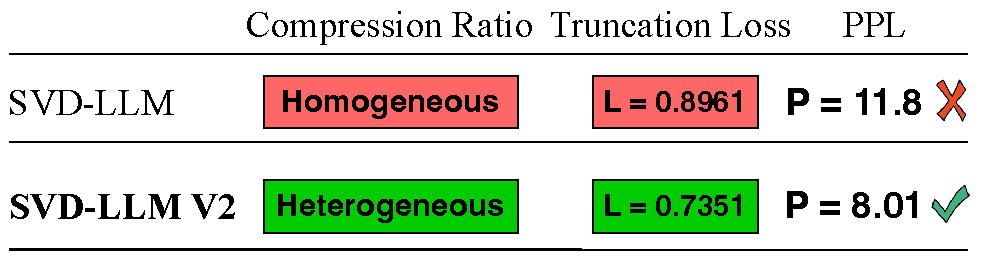
\includegraphics[width=0.48\textwidth]{Figures/Motivation.pdf}
\caption{Comparison between \sysname and SVD-LLM. We randomly select a weight matrix from LLaMA-3 8B and compare the normalized truncation loss and perplexity (PPL) under 20\% compression ratio. }
\label{fig:motivation}
\end{figure}

Low-rank approximation, such as Singular Value Decomposition (SVD) is also an effective technique for compressing LLMs. Compared with quantization and unstructured pruning, SVD compression is more hardware-friendly. 
%
Recently, a few SVD-based LLM compression methods
% such as FWSVD~\citep{DBLP:conf/iclr/HsuHCLSJ22}, ASVD~\citep{DBLP:journals/corr/abs-2312-05821} and SVD-LLM~\citep{DBLP:journals/corr/abs-2403-07378} 
have been proposed. At a high level, these methods all focus on reducing the truncation loss during SVD compression to reserve accuracy.  
%
Specifically, FWSVD~\citep{DBLP:conf/iclr/HsuHCLSJ22} reduces truncation loss by estimating weight importance and preserving more important weights.
%
ASVD~\citep{DBLP:journals/corr/abs-2312-05821} injects a scaling matrix to reduce the truncation loss but was not able to achieve theoretical minimum truncation loss at each LLM layer. 
%
SVD-LLM~\citep{DBLP:journals/corr/abs-2403-07378}, on the other hand, fills this gap by proposing a whitening matrix that obtains theoretical minimum truncation loss at each LLM layer, demonstrating superior performance.  


% However, these methods often exhibit severe performance degradation.
%However, due to XXX, SVD-LLM fails to obtain the theoretical minimum truncation loss in practice. 
%
Despite such advantage, SVD-LLM has two limitations.
%
First, SVD-LLM applies a homogeneous compression ratio to all the weight matrices. This coarse-grained setup unfortunately overlooks the heterogeneity of weight redundancy across different LLM layers. 
%
Second, SVD-LLM utilizes Cholesky decomposition for weight truncation. However, Cholesky decomposition requires the matrix being decomposed to be positive-definite, a condition that is challenging to fulfill in practice. Moreover, Cholesky decomposition introduces numerical instability throughout its iterative process. 
%
As a consequence, SVD-LLM
could still lead to high truncation loss in practice.
%, even under a low compression ratio\footnote{The compression ratio refers to the percentage of model parameters reduced through compression.}. 
%As a result, given the input activation, the output between the compressed weight matrices and the original ones in the LLM will be significantly different, making the compressed LLM behave much poorer than the original LLM. 
%

% \newpage
In this paper, we propose \sysname, a SVD-based post-training LLM compression method that effectively addresses the two limitations of SVD-LLM.
%
First, to address the heterogeneity of weight redundancy across layers, \sysname uses the theoretical truncation loss of
weight matrices at each layer as the guidance to assign a unique compression
ratio to each weight matrix based on its type at different layers.
%allocates compression ratios among the weight matrices in different layers.
%to remove the necessity for the decomposed matrix to be positive-definite and to enhance numerical stability,
Second, \sysname substitutes the Cholesky decomposition with two rounds of SVD for weight truncation, which we prove to achieve the theoretical minimum truncation under the optimized compression ratio.
%
In doing so, \sysname is able to achieve better perplexity with lower truncation loss than SVD-LLM (\cref{fig:motivation}).

%For a better demonstration, we compare the truncation loss and the final performance of SVD-LLM~\citep{DBLP:journals/corr/abs-2403-07378} and \sysname on LLaMA-3 8B. As shown in~\cref{fig:motivation}, \sysname achieves a better perplexity with lower truncation loss than SVD-LLM.

We evaluate \sysname on ten datasets covering various language modeling, classification, and generation tasks as well as five LLMs with various backbones and scales. Our results demonstrate the superiority of \sysname with three key findings:


\vspace{-2mm}
\begin{itemize}
    \item \sysname consistently outperforms state-of-the-art SVD-based LLM compression methods across all ten datasets and five LLMs.
    %, achieving over 99\% lower perplexity under 40\% compression ratios and above.
    \vspace{-2mm}
    \item  \sysname outperforms state-of-the-art structured pruning-based LLM compression methods with up to 28\% lower perplexity under 7 GB memory budget. 
    %
    When comparing to state-of-the-art 1-bit quantization-based LLM compression methods, \sysname outperforms PB-LLM and achieves 5\% lower perplexity. 
    %compressing a 16-bit LLM, \sysname achieves performance comparable to using 1-bit post-training quantization techniques under the same memory budget. 
    %
    Moreover, by combining with 2-bit quantization, \sysname is able to outperform 1-bit BiLLM, demonstrating the promise of combining SVD and quantization-based methods for advancing the frontier of post-training LLM compression.
    %when compressing a 2-bit LLM, \sysname surpasses the performance of the state-of-the-art 1-bit quantization with up to 69\% lower perplexity.
    \vspace{-2mm}
    \item LLMs compressed by \sysname achieve inference speedup on real hardware. In particular, LLMs compressed by \sysname are able to achieve a throughput speedup of up to 2.71$\times$ compared to the original LLMs on a single NVIDIA A100 GPU.
\end{itemize}

\section{Related Work}
\label{sec:related_works}
\vspace{-1mm}


\begin{figure*}[t]
\centering
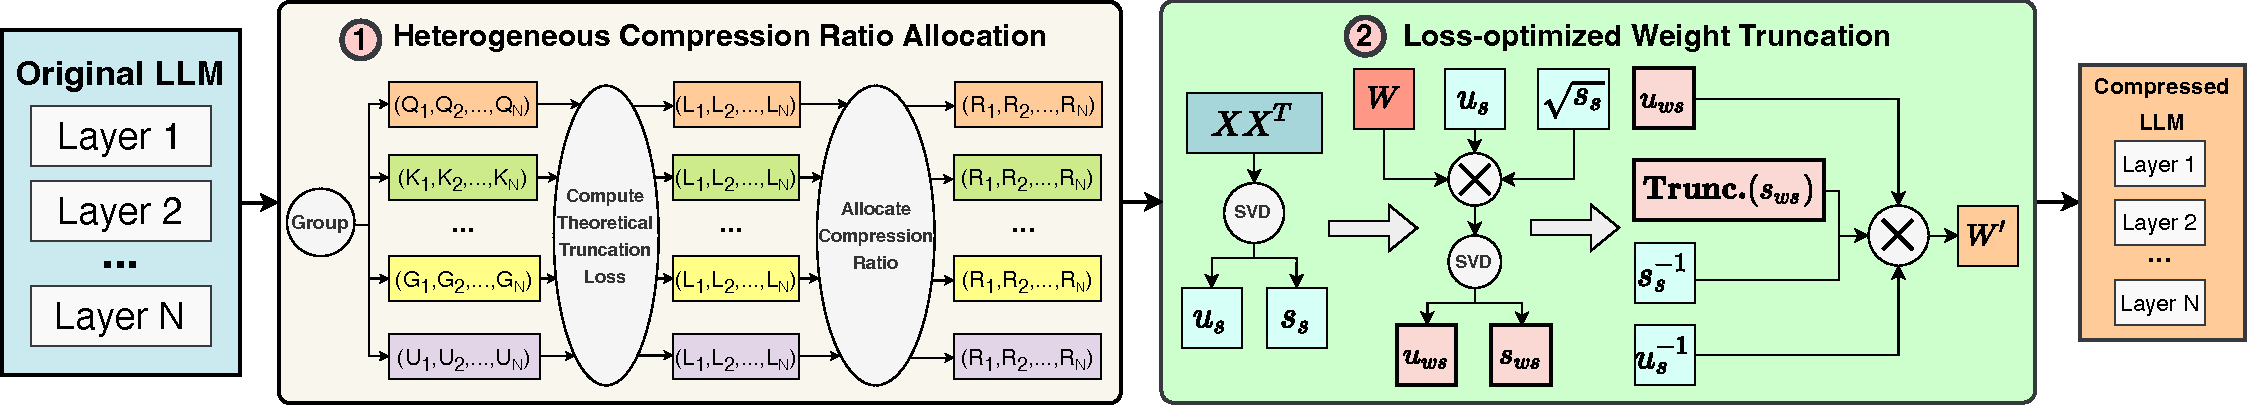
\includegraphics[width=1\textwidth]{Figures/Framework.pdf}
\caption{Overview of \sysname.}
\label{fig:framework}
\end{figure*}


\subsection{Large Language Model Compression}
\label{subsc:large_language_model_compression}
Large Language Models (LLMs) typically contain billions of parameters, making traditional model compression techniques impractical due to the need for resource-intensive retraining. To address this, post-training methods that bypass retraining during compression have been developed. These methods generally fall into four categories: unstructured pruning, structured pruning, quantization, and low-rank approximation. 
%
Unstructured pruning~\citep{DBLP:conf/icml/FrantarA23} sets the individual weight values to zero without changing the overall architecture. However, its irregular sparsity is feasible only for speedups or memory savings on certain hardware. 
%
In contrast, structured pruning~\citep{DBLP:conf/nips/MaFW23,DBLP:conf/iclr/AshkboosCNHH24,DBLP:journals/corr/abs-2406-10594} removes entire channels from LLMs, simplifying hardware implementation but often suffering from accuracy degradation. 
%
Quantization~\citep{DBLP:journals/corr/abs-2210-17323,DBLP:journals/corr/abs-2411-07762} reduces the precision of the weight matrices for compression. However, it often fails to provide the desired inference speedups~\citep{DBLP:journals/corr/abs-2405-04532} and offers a limited range of compression options—typically between 2 to 8 bits—which hinders optimal memory utilization. Recent efforts~\citep{DBLP:conf/iclr/YuanSD24, DBLP:conf/icml/HuangLQLZ0M024} have explored 1-bit post-training quantization. Nevertheless, these approaches still suffer from accuracy drop, indicating that 1-bit quantization is still challenging in LLM compression.

\subsection{SVD for LLM Compression}
Singular Value Decomposition (SVD) reduces matrix sizes by truncating the smallest singular values. It then constructs two smaller, lower-rank matrices to approximate the original matrix~\citep{GOLUB1987317}. SVD is also feasible for LLM~\citep{DBLP:conf/iclr/HsuHCLSJ22, DBLP:journals/corr/abs-2312-05821, DBLP:journals/corr/abs-2403-07378,DBLP:journals/corr/abs-2408-09632}. To ensure better compression performance, existing post-training SVD-based LLM compression methods attempt to lower the truncation loss $L$ in the form of Frobenius norm as follows during LLM compression:

\begin{equation}
    L = ||WX-W'X||_F 
    \label{eq:t1}
\end{equation}

\noindent where $W$ is the weight matrix of the original LLM, $X$ is the activation of $W$, and $W'$ is the compressed low-ranking weight matrix. 
% %
% and many SVD-based compression techniques have been proposed. 
For example,
%\citet{DBLP:conf/iclr/HsuHCLSJ22} propose FWSVD which introduces Fisher information to weigh the importance of parameters.
%
\citet{DBLP:journals/corr/abs-2312-05821} propose ASVD, which scales the weight matrix using a diagonal matrix to normalize the impact of input channels on the weights to reduce the truncation loss. 
%
\citet{DBLP:journals/corr/abs-2403-07378} make further advancement by whitening the input matrix to mitigate its impact on SVD truncation with the guarantee of minimal theoretical truncation loss. 
%
Despite these progresses, existing methods still suffer from high truncation loss in practice, leading to accuracy degradation.
%, which severely hinders their real-world application.
\section{SVD-LLM V2}
\label{sec:methodology}

% \begin{figure*}[t]
% \centering
% 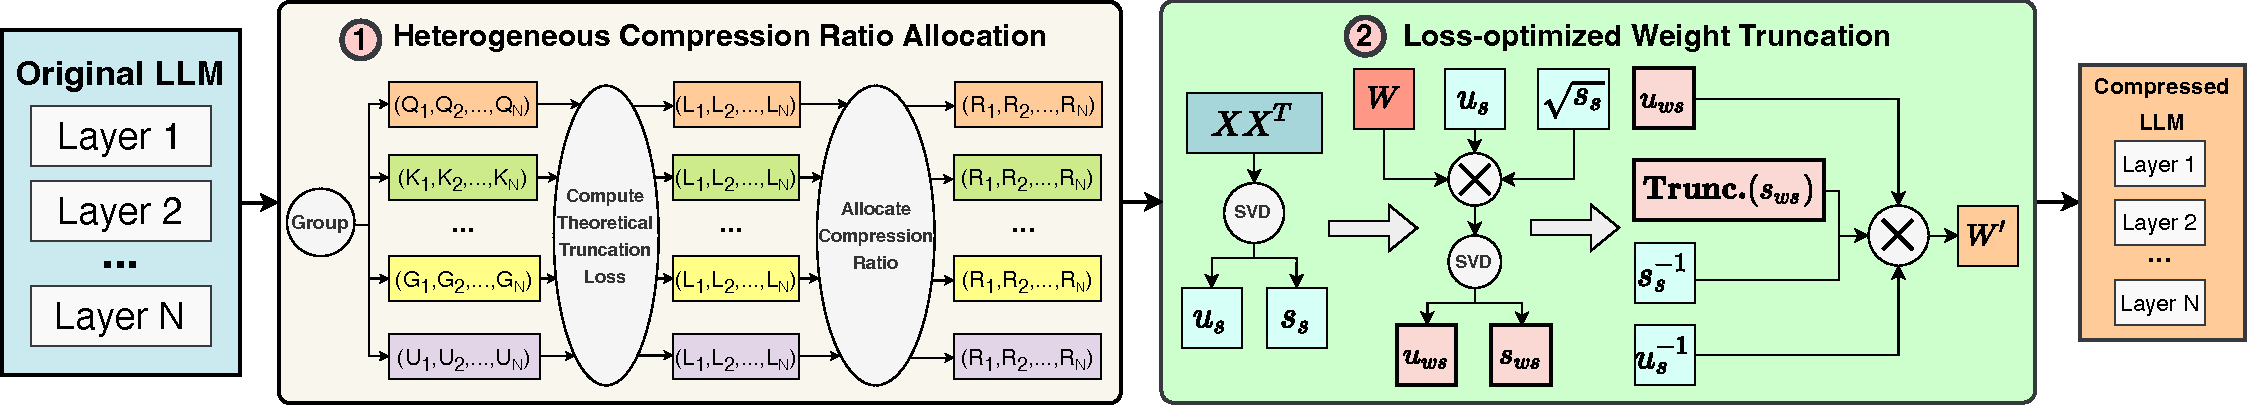
\includegraphics[width=1\textwidth]{Figures/Framework.pdf}
% \caption{Overview of \sysname.}
% \label{fig:framework}
% \end{figure*}

% \begin{figure}[htbp]
%     \centering
%     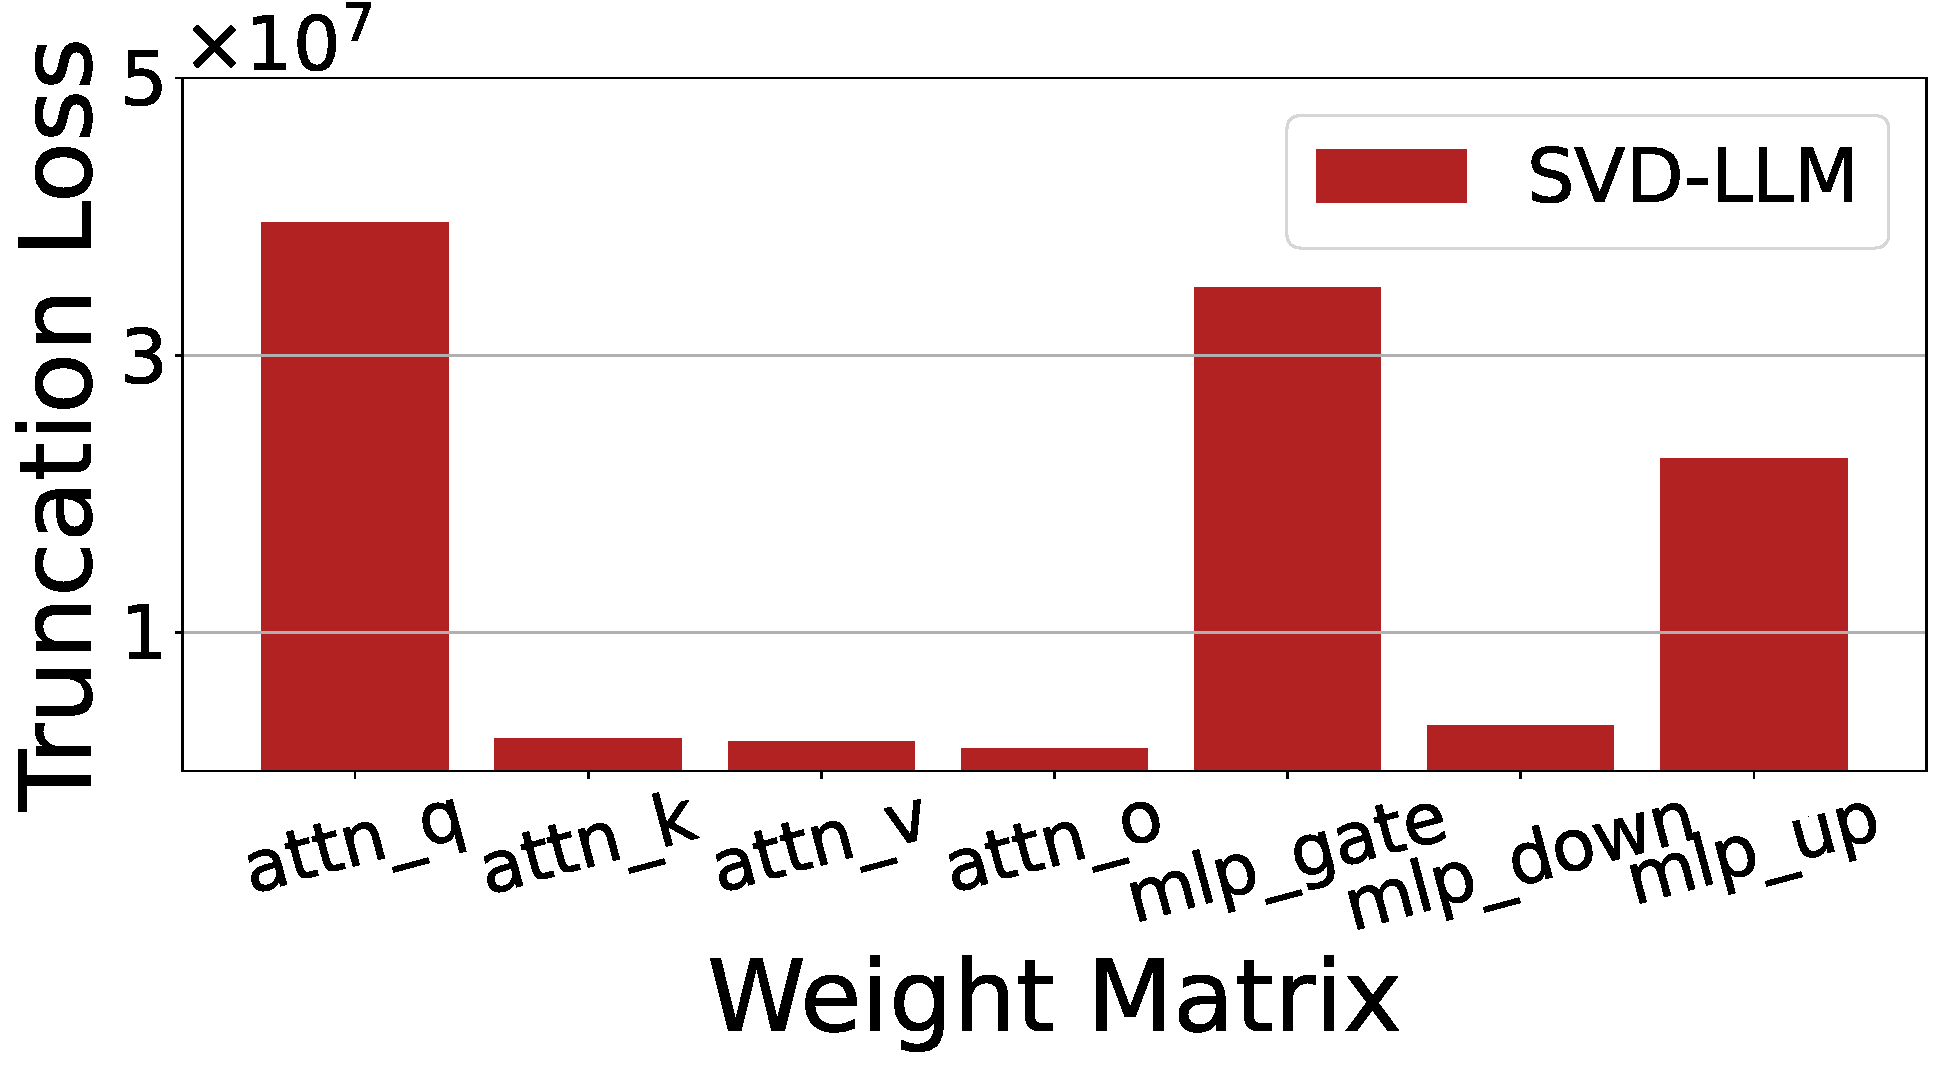
\includegraphics[width=0.45\textwidth]{Figures/Motivation_2.pdf}
%     \caption{Truncation loss by SVD-LLM of weight matrices in one randomly selected decoding layer in LLaMA-3 8B on WikiText-2 under 50\% compression ratio.}
%     \label{fig:motivation_2}
% \end{figure}

%In this section, we present the main design of our proposed \sysname for compressing LLMs. 
\cref{fig:framework} provides an overview of \sysname. 
%
Specifically, \sysname groups the weight matrices across all the layers in the original LLM by type, such as query ($Q$) and key ($K$) in attention blocks, and Gate ($G$) and Up ($U$) in MLP blocks. It then computes the theoretical truncation loss of the weight matrices and assigns a unique compression ratio to each weight matrix within each group based on the computed truncation loss.
%After obtaining all compression ratios across the weight matrices, 
Lastly, \sysname performs loss-optimized weight truncation to obtain the compressed LLM.
%
Below, we describe the details of the two main components of \sysname: (1) heterogeneous compression ratio allocation and (2) loss-optimized weight truncation. 
%
% The pseudocode of \sysname is provided in \xin{xxx}.

% \subsection{Motivation}
% \label{subsec:motivation}
% % \xin{Loss figure (loss increases significantly with ratio}
% To ensure better compression performance, many recent post-training SVD-based LLM compression works~\citep{DBLP:conf/iclr/HsuHCLSJ22, DBLP:journals/corr/abs-2312-05821, DBLP:journals/corr/abs-2403-07378} attempt to lower the truncation loss $L$ in the form of Frobenius norm as follows during their LLM compression:

% \begin{equation}
%     L = ||WX-W'X||_F 
%     \label{eq:t1}
% \end{equation}

% \noindent where $W$ is the weight matrix of the original LLM, $X$ is the activation of $W$, and $W'$ is the compressed low-ranking weight matrix.

% Although the state-of-the-art method SVD-LLM~\citep{DBLP:journals/corr/abs-2403-07378} has theoretically guaranteed the alignment between truncated singular values and the corresponding truncation loss, which reduces the truncation loss and significantly enhances the compressed LLMs' performance, it still fails to ensure the minimization of the truncation loss during the SVD compression. 
% %
% For a better demonstration, we randomly select one of the decoding layers in LLaMA-3 8B and compute the corresponding truncation loss of all weight matrices under 50\% compression ratio. As shown in~\cref{fig:motivation_2}, all the weight matrices suffer severely from the huge truncation loss. For the weight matrices in other decoding layers, we also observe a similar trend.
% %
% As a result, the output $W'X$ computed by the compressed weight matrix $W$ significantly deviates from $WX$ computed by the original weight matrix $W$, causing the final performance of compressed LLM to drop significantly. Therefore, it is still necessary to design a new method with a better ability to minimize truncation loss.

\subsection{Heterogeneous Compression Ratio Allocation}
\label{subsec:dynamic_ratio_allocation}
\noindent \textbf{Motivation:} Since different weight matrices in LLMs often exhibit different levels of redundancy, applying a homogeneous compression ratio to all the weight matrices would incur high truncation loss for those with low redundancy~\citep{DBLP:journals/corr/abs-2406-10594,DBLP:journals/corr/abs-2406-15786,DBLP:journals/corr/abs-2407-19126}. 
%
To demonstrate this, we use SVD-LLM to measure the truncation loss of the query matrix across different layers in LLaMA-3 8B on WikiText-2 dataset with 50\% compression ratio. 
%
As shown in~\cref{fig:layer}, the truncation loss varies at different layers. For example, the query matrix in the 27th layer has a much higher truncation loss than that of the first layer, indicating the 27th layer should be compressed under a smaller compression ratio, while a larger compression ratio should be applied to the first layer. 
%
However, existing SVD-based LLM compression methods either overlook this variation or require resource-intensive operations to determine the specific compression ratios, making them impractical for compressing LLMs at larger scales. 
%
Therefore, it is essential to develop a more efficient approach to apply different compression ratios at different weight matrices to reduce the truncation loss.


\begin{figure}[t]
    \centering
    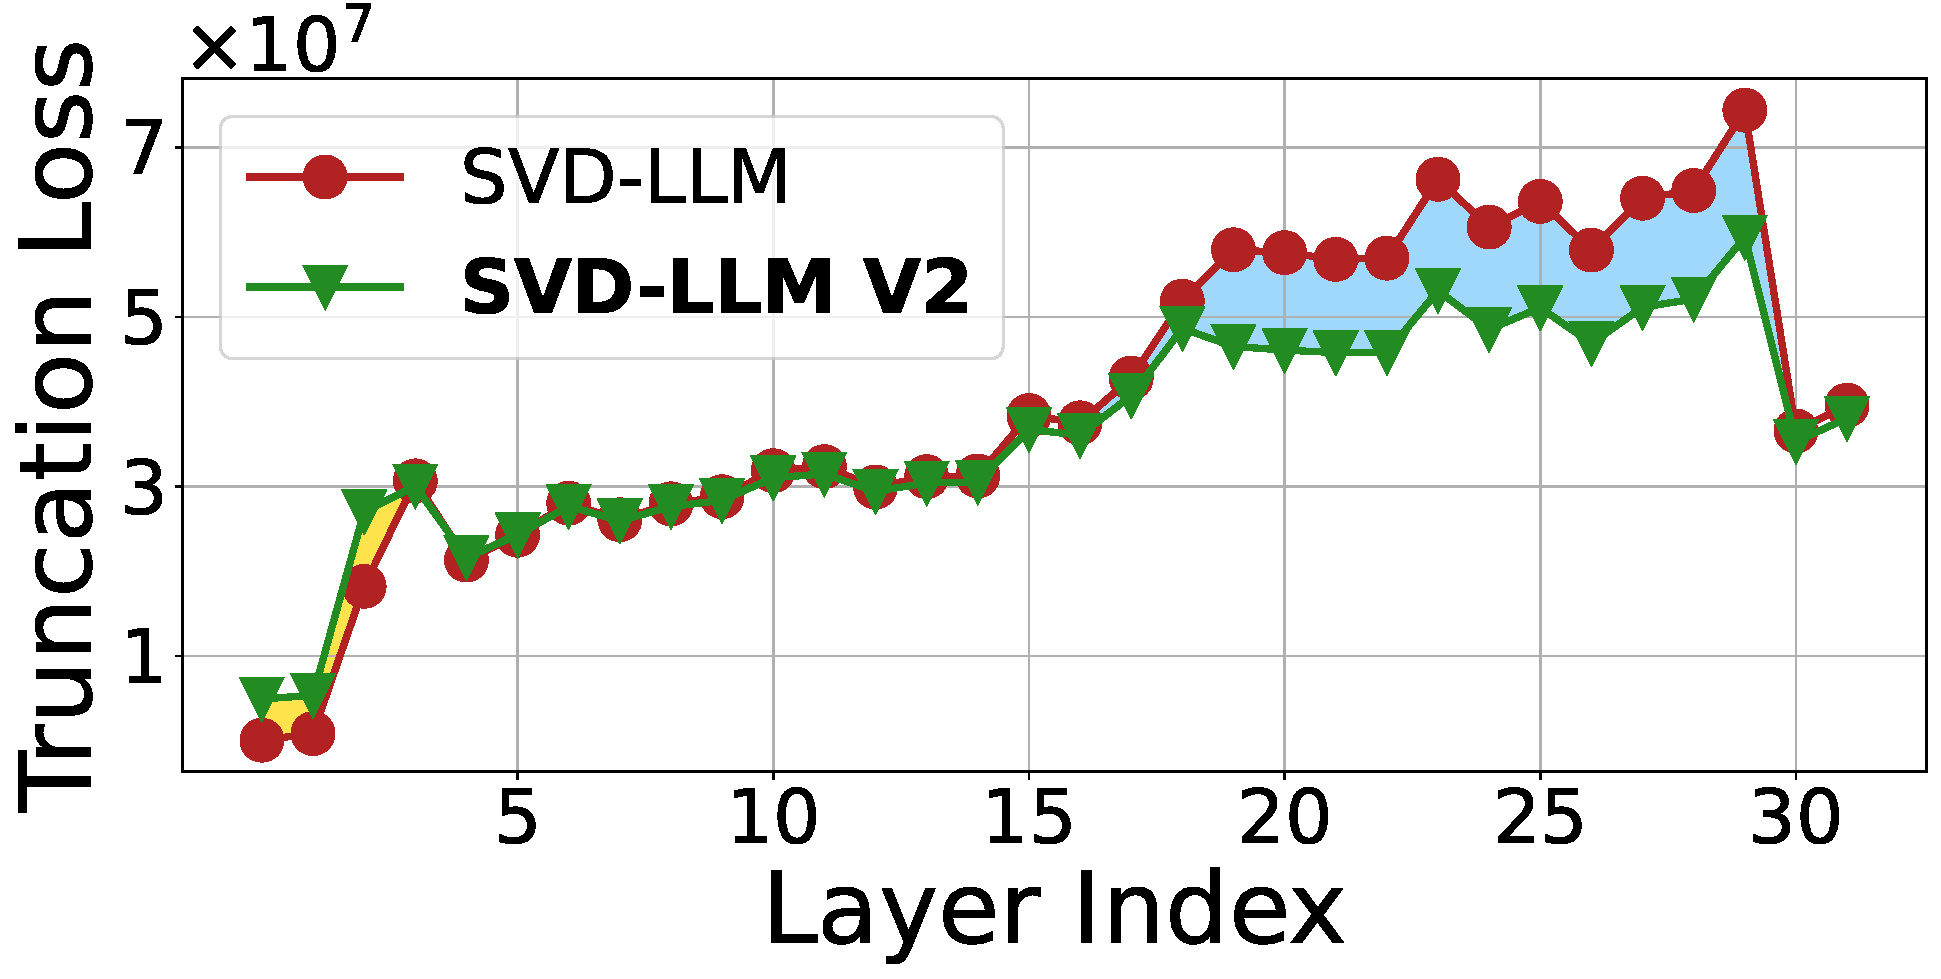
\includegraphics[width=0.45\textwidth]{Figures/Layer.pdf}
    \caption{Comparison between SVD-LLM and \sysname on the truncation loss of the query weight matrix across different layers in LlaMA-3 8B on WikiText-2 dataset with 50\% compression ratio.}
    \label{fig:layer}
\end{figure}


\begin{algorithm}[t]
\captionsetup{font=small}
\caption{Pseudocode of Heterogeneous Compression Ratio Allocation in \sysname}
\small
\begin{algorithmic}[1] % The number [1] tells LaTeX to number each line
\Statex \textbf{Input:} $M$: Original LLM 
\Statex \hspace{3em} $x$: Input activation
\Statex \hspace{3em} $R$: Target compression ratio
\Statex \textbf{Output:} $R_d$: A list of allocated compression ratios
% \setcounter{ALG@line}{0}  % 重置行号计数器，从0开始
\Procedure{Ratio\_Allocation}{$M, S, R$} % Algorithm name and parameters
    \State $G \gets \boldsymbol{\operatorname{Group}}(M)$  \Comment{Group the weight by types}
    \State $R_d \gets \emptyset$ \Comment{Initialize the compression ratio list} 
        \For{$g$ \textbf{in} $G$}
        \State $L_G \gets \emptyset$ \Comment{Initialize the loss list in the group} 
            \For{$w$ \textbf{in} $g$}
            % \State $w' \gets \boldsymbol{\operatorname{Weight\_Truncation}}(w, x, R)$
                \State $L_{min} \gets \boldsymbol{\operatorname{Theoretical\_Loss}}(w, x, R)$
                \State $L_{G} \gets L_{G} \cup L_{min}$ 
            \EndFor
            \State $L_{G} \gets 1 / \boldsymbol{\operatorname{Log}}(L_{G})$ \Comment{Normalize $L_G$}
            \State $r \gets \boldsymbol{\operatorname{Len}}(L_{G}) \times R\times L_{min} / \boldsymbol{\operatorname{Sum}}(L_{G})$
            \State $R_d \gets R_d \cup r$ \Comment{Append $r$ to the list $R_d$} 
        \EndFor
    \State \Return{$R_d$}
\EndProcedure
\end{algorithmic}
\label{algo:compression_ratio}
\end{algorithm}

\noindent \textbf{Key Design:} 
%
The pseudocode of the heterogeneous compression ratio allocation is listed in~\cref{algo:compression_ratio}. 
%
Specifically, 
% to calculate the truncation loss more efficiently and accurately, 
% \sysname applies a whitening matrix $S$,  as done in SVD-LLM~\citep{DBLP:journals/corr/abs-2403-07378} to align the truncation loss with singular values. 
% We follow the same procedure in SVD-LLM to construct a calibration set $X$ and compute the whitening matrix $S$ with the Choloesky decompostion of $XX^T$. In this way, the truncation loss $L$ to truncate the multiple singular values $(\sigma_0, \sigma_1, \cdots, \sigma_k)$ could easily be obtained by $\sqrt{\sum_{i=0}^k \sigma_i^2}$. 
% \sysname applies its own loss-optimized weight truncation, which is more accurate and stable than the truncation done in SVD-LLM, as described in~\cref{subsec:loss_optimized_weight_truncation} to pre-compress the weight matrix under a given compression ratio $R$ and compute its corresponding truncation loss.
%
given that different types of weight matrices, such as query ($Q$) and key ($K$) in attention blocks, and Gate ($G$) and Up ($U$) in MLP blocks play different roles in an LLM, 
%it is inappropriate to consider them together for compression ratio allocation. 
%Therefore, given the specific compression ratio $R$, 
\sysname first groups the weight matrices across all the layers in the original LLM according to their types. 
%
Next, \sysname computes the theoretical minimum truncation loss of the weight matrices, i.e., $L_{min} = ||C-C'||_F$, where $C$ is the original matrix of $WX$ and $C'$  is its compressed version by SVD, respectively. It then inverses and normalizes $L_{min}$ by $1/\text{Log}(L_{min})$.
%
Finally, given the target model compression ratio $R$, the compression ratio of each weight matrix within a group is determined as $ \text{Len}(L_{G}) \times R \times L_{min} / \text{Sum}(L_{G})$, where $L_{G}$ denotes the list of theoretical truncation loss for all matrices within the same group, $\text{Len}(L_{G})$ denotes the group size and $\text{Sum}(L_{min})$ denotes the sum of the loss within this group. 
%
In this way, \sysname bypasses the need to measure end-to-end perplexity to determine compression ratios, as done in ASVD and is time-consuming. Instead, it utilizes truncation loss, which is easy to obtain and thereby enhancing the efficiency of the algorithm.
%
As shown in~\cref{fig:layer}, with the proposed heterogeneous compression ratio allocation scheme, \sysname effectively reduces the truncation loss (the blue area) with only a small increase of several small truncation losses (the yellow area).

% After determining the specific compression ratio for each weight matrix in the LLM, \sysname incorporates a loss-optimized weight truncation to truncate the weight matrices based on their assigned compression ratios to obtain the compressed LLM.
%the next step is to apply the real truncation on the weights  
%
In the next section, we describe the details of the proposed loss-optimized weight truncation.  
%
% \vspace{-3mm}



\subsection{Loss-optimized Weight Truncation}
\label{subsec:loss_optimized_weight_truncation}
%
\noindent \textbf{Motivation:} 
After determining the specific compression ratio for each weight matrix in the LLM, the next step is to truncate the weights according to their assigned compression ratios. 
%
To reduce truncation loss $L= ||WX-W'X||_F$ during SVD compression, SVD-LLM first constructs the whitening matrix $S$ by applying Cholesky decomposition on $XX^T$. It then performs SVD and truncation on $WS$. Although SVD-LLM has been theoretically proven to achieve the lowest truncation loss at a given compression ratio, our empirical study shows that its actual truncation loss is frequently above the theoretical minimum. This is mainly due to the numerical instability involved in performing the Cholesky decomposition on a large-scale matrix during truncation. Moreover, the Cholesky decomposition requires $XX^T$ to be positive definite, which is often hard to satisfy.
%during compression.

%
To demonstrate this, we randomly select two weight matrices, $A$ and $B$, in LLaMA-3 8B and compute their truncation loss by SVD-LLM using 256 randomly selected data in the C4 dataset under compression ratios 20\% and 60\%. As shown in~\cref{tab:loss_comparison}, because $XX^T$ is not positive definite, SVD-LLM fails to compress matrix $A$. For matrix $B$, even when the compression ratio is as low as 20\%, SVD-LLM still achieves a larger truncation loss in practice than in theory, and this difference even increases with increasing compression ratio. 

SVD-based LLM compression methods such as Balco~\citep{DBLP:journals/corr/abs-2405-10616} have been proposed that utilize pooled covariance matrices to precisely estimate the feature distribution to reduce truncation loss. However, these methods cannot guarantee their theoretical optimality during SVD truncation. 
%
Therefore, it is necessary to design a new way to optimize the truncation loss for SVD compression. 

\losscomparisonTable
\vspace{2mm}

% \begin{figure}[htbp]
%     \centering
%     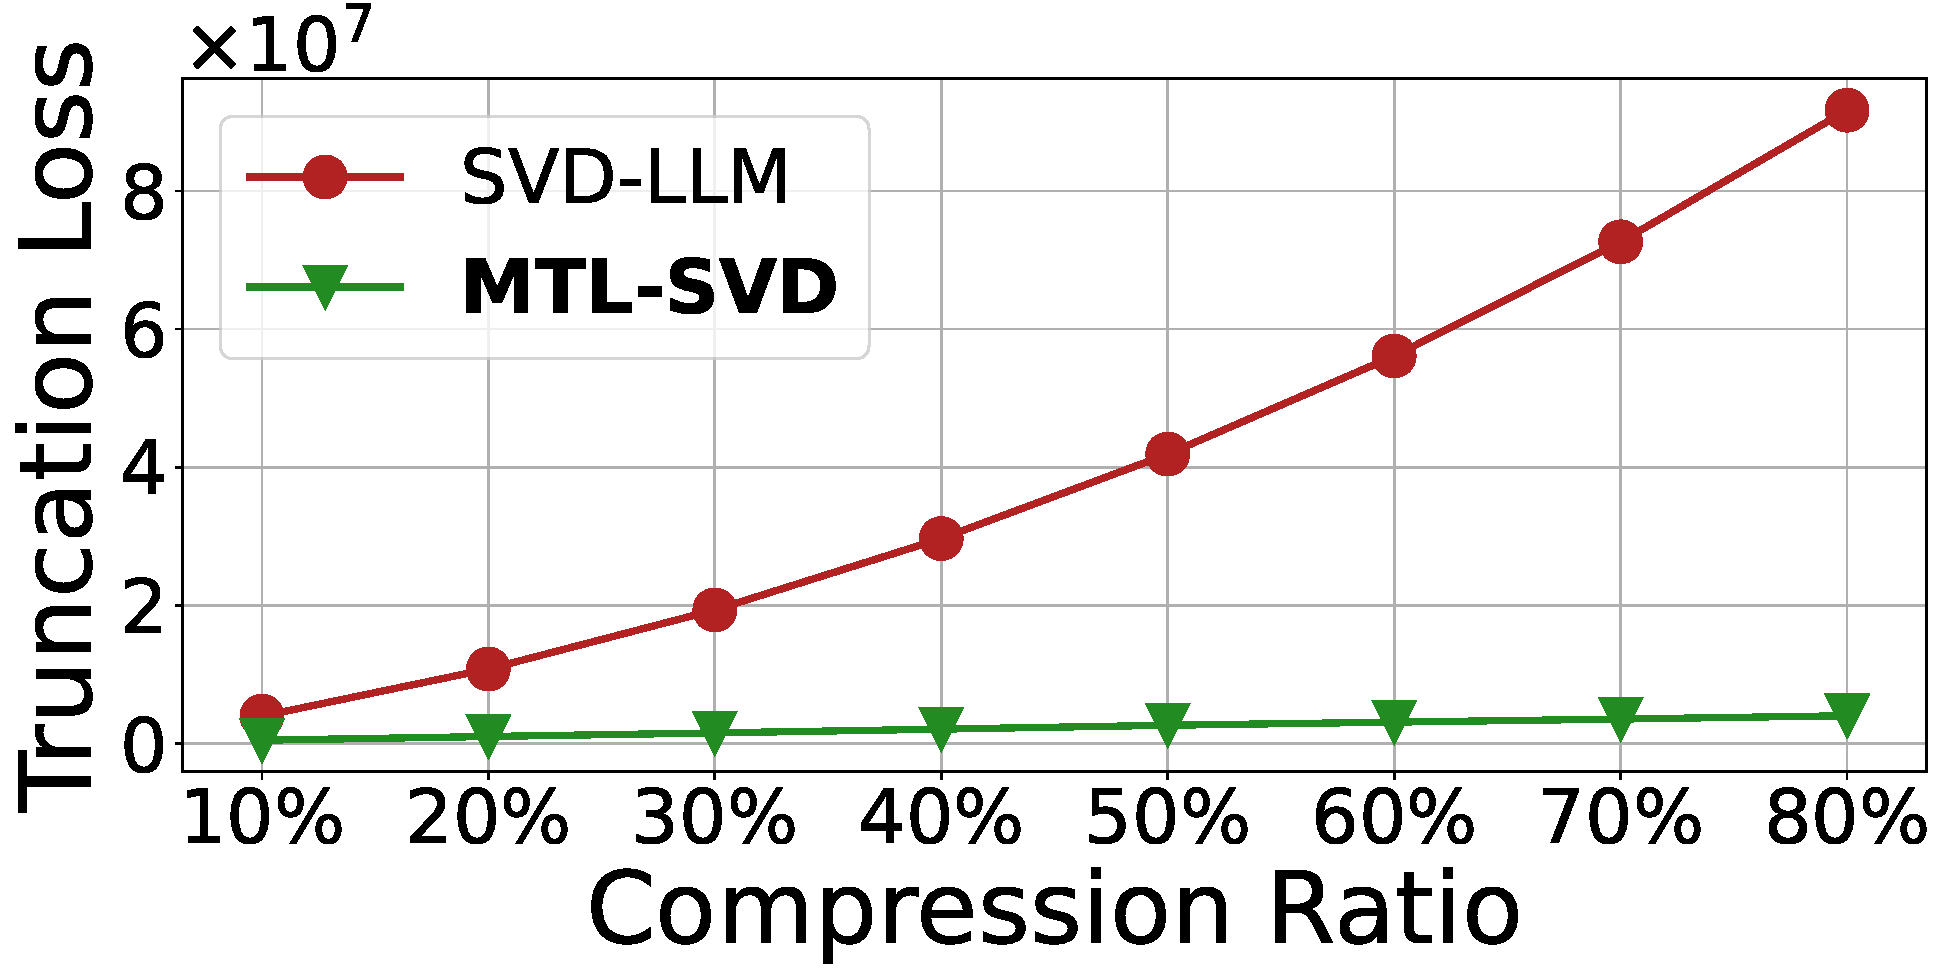
\includegraphics[width=0.45\textwidth]{Figures/Loss.pdf}
%     \caption{Truncation loss by SVD-LLM and \sysname of the weight matrix randomly selected in LLaMA-3 8B on WikiText-2 under different compression ratios.}
%     \label{fig:loss}
% \end{figure}

\begin{algorithm}[t]
\captionsetup{font=small}
\caption{Pseudocode of Loss-optimized Weight Truncation in \sysname}
\small
\begin{algorithmic}[1] % The number [1] tells LaTeX to number each line
\Statex \textbf{Input:} $W$: Original weight matrix 
\Statex \hspace{3em} $X$: Input activation
\Statex \hspace{3em} $R$: Target compression ratio
\Statex \textbf{Output:} $W'$: Compressed weight matrix
% \setcounter{ALG@line}{0}  % 重置行号计数器，从0开始
\Procedure{Weight\_Truncation}{$W, X, R$} % Algorithm name and parameters
    \State $S \gets XX^T$  \Comment{Construct matrix $S$ from $X$}
    \State $U_s, S_s, V_s \gets \boldsymbol{\operatorname{SVD}}(S)$ \Comment{Perform SVD on matrix $S$} 
    \State $D \gets W\times U_s \times \sqrt{S_s}$  \Comment{Construct matrix $D$}
    \State $U_{ws}, S_{ws}, V_{ws} \gets \boldsymbol{\operatorname{SVD}}(D)$ \Comment{Perform SVD on matrix $D$}
    \State $T_s \gets \boldsymbol{\operatorname{Truncate}}(S_{ws}, R)$ \Comment{Perform SVD truncation on matrix $S_{ws}$ based on compression ratio $R$}
    \State $W' \gets U_{ws}\times T_s \times S_{s} ^{-1}\times U_{s}^{-1}$ \Comment{Construc $W'$}
    \State \Return{$W'$}
\EndProcedure
\end{algorithmic}
\label{algo:weight_truncation}
\end{algorithm}




\noindent \textbf{Key Design:}
The pseudocode of the proposed loss-optimized weight truncation is provided in~\cref{algo:weight_truncation}. Different from SVD-LLM, \sysname bypasses the Cholesky decomposition, resulting in a more straightforward process with improved numerical stability. Specifically, given the input activation $X$, \sysname conducts SVD on $XX^T$ to obtain the decomposed matrices $U_s, S_s, V_s$, where $S_s$ is the diagonal matrix with singular values. It then conducts another round of SVD on $W\times U_s\times \sqrt{S_s}$ to obtain $U_{ws}, S_{ws}, V_{ws}$. The final compressed weight matrix $W'$ can be obtained via $U_{ws}\times \boldsymbol{\operatorname{Trunc.}}(S_{ws}) \times S_{s} ^{-1}\times U_{s}^{-1} $, where $\boldsymbol{\operatorname{Trunc.}}(C)$ denotes the rank-k truncation of matrix $C$ during SVD compression.

In the following, we provide a theoretical proof on why such truncation offers the same theoretical minimum truncation loss as SVD-LLM.

\begin{theorem}
\label{thm:whitening}
If $U_s, S_s, V_s$ are obtained by SVD decomposition of $XX^T$ and $U_{ws}, S_{ws}, V_{ws}$ are obtained by SVD decomposition of $W\times U_s\times \sqrt{S_s}$, the compressed weight matrix $W' = U_{ws}\times \boldsymbol{\operatorname{Trunc.}}(S_{ws}) \times V_{ws} \times \sqrt{S_{s}}^{-1} \times U_{s}^{-1}$ ensures the theoretical minimum truncation loss.
\end{theorem}

\begin{proof}
\label{proof:truncation}
Since $XX^T$ is the symmetric matrix, suppose that the singular vectors and values of input activation $X$ is $U_x, S_x, V_x$, we have $U_s = U_x$ and $\sqrt{S_s} = S_x$. Suppose $S = U_s\times \sqrt{S_s}$, thus $S^{-1} = \sqrt{S_{s}}^{-1} \times U_{s}^{-1}$, and we have:

 % \vspace{-2mm}
{\small
\begin{equation}
    \begin{aligned}
        &S^{-1} X = \sqrt{S_{s}}^{-1} U_{s}^{-1} X = S_{x}^{-1} U_{x}^{-1} X\\
        &= S_{x}^{-1} U_{x}^{-1} U_x S_x V_x = Vx
    \end{aligned}
\label{formula:derive}
\end{equation}
}

\noindent Therefore, $S^{-1}\times X$ is orthogonal and $||A\times S^{-1}\times X||_F = ||S^{-1}\times X||_F$, and the final truncation loss could be derived as:

%\vspace{-4mm}
{\small
\begin{equation}
    \begin{aligned}
        &L^2 =||W X-W^{\prime} X||_F^2 \\
        &= ||WSS^{-1}X - U_{ws}\times \boldsymbol{\operatorname{Trunc.}}(S_{ws}) \times V_{ws} \times S^{-1} X||_F^2\\
        &= ||(WS - U_{ws}\times \boldsymbol{\operatorname{Trunc.}}(S_{ws}) \times V_{ws})S^{-1}X||_F^2\\
        &= ||WS - U_{ws}\times \boldsymbol{\operatorname{Trunc.}}(S_{ws}) \times V_{ws}||_F^2\\
        &= ||\boldsymbol{\operatorname{SVD}}(WS)||_F^2 = ||\boldsymbol{\operatorname{SVD}}(W\times U_x\times S_x)||_F^2\\
        & = ||\boldsymbol{\operatorname{SVD}}(W\times U_x\times S_x\times V_x)||_F^2\\
        & = ||\boldsymbol{\operatorname{SVD}}(WX)||_F^2 = L_{min} ^2
    \end{aligned}
\label{formula:loss_1}
\end{equation}
}

\noindent Therefore, the designed SVD truncation ensures the theoretical minimum truncation loss.
\end{proof}

For a better demonstration, we also implement the new loss-optimized weight truncation by \sysname on LLaMA-3-8B. As shown in~\cref{tab:loss_comparison}, \sysname achieves better numerical stability and lower truncation loss than SVD-LLM.
% demonstrating the effectiveness of our proposed loss-minimized weight truncation strategy.

% \noindent Therefore, we have: 

% % \vspace{-2mm}
% {\small
% \begin{equation}
%     \begin{aligned}
%         &L^2 =||W X-W^{\prime} X||_F^2 \\
%         & =\sum_{j=1}^r \sum_{i=1}^r \sigma_i \sigma_j \boldsymbol{\operatorname{trace}}(Mu_i v_i^T v_j u_j^TM^T)\\
%         & =  \sum_{i=1}^r\sigma_i^2\boldsymbol{\operatorname{trace}}(Mu_iu_i^TM^T)\\
%         & =  \sum_{i=1}^r\sigma_i^2||Mu_i||_F^2 \leq ||M||_F^2\sum_{i=1}^r\sigma_i^2
%     \end{aligned}
% \label{formula:loss_2}
% \end{equation}
% }

% \noindent Therefore, we have $L\leq\sqrt{||M||_F^2\sum_{i=1}^r \sigma_i^{2} }$.


% Therefore, we could  indirectly minimize the truncation loss through lowering this upper-bound. The gradient of $L$ can be calculated as:

% % \vspace{-4mm}
% {\small
% \begin{equation}
%     \begin{aligned}
%         &\nabla_M L^2=\nabla_M (||M||_F^2\cdot \sum_{i=1}^r\sigma_i^2)\\
%         &=\nabla_M||M||_F^2\cdot \sum_{i=1}^r\sigma_i^2 + ||M||_F^2 \nabla_M\sum_{i=1}^r\sigma_i^2\\
%         &=\sum_{i=1}^r\sigma_i^2 \cdot 2M - 2||M||_F^2 \cdot \sum_{i=1}^r\sigma_i (M^{-1})^TU_iV_i^T(WS)^T
%     \end{aligned}
% \label{formula:gradient}
% \end{equation}
% }

% \noindent where $U_i$ and $V_i$ are the left and right singular vectors corresponding to the $i$-th singular value $\sigma_i$. Therefore, the gradient is easy to obtain, which makes it convenient for us to apply some existing optimization algorithms\footnote{In our paper, we use L-BFGS~\citep{Nash1991ANS} algorithms as the default} with the computed gradient to further minimize the truncation loss. Different from directly optimizing $W'$ based on the original truncation loss $L = ||WX-W'X||_F$ that requires storing every large-scale activation matrix $X$, which is impractical in the post-training LLM compression scenario, optimizing with gradient computed from \cref{formula:gradient} does not need to store activation, which is more efficient and feasible.

% \begin{figure}[htbp]
% % \vspace{-2mm}
%     \centering
%     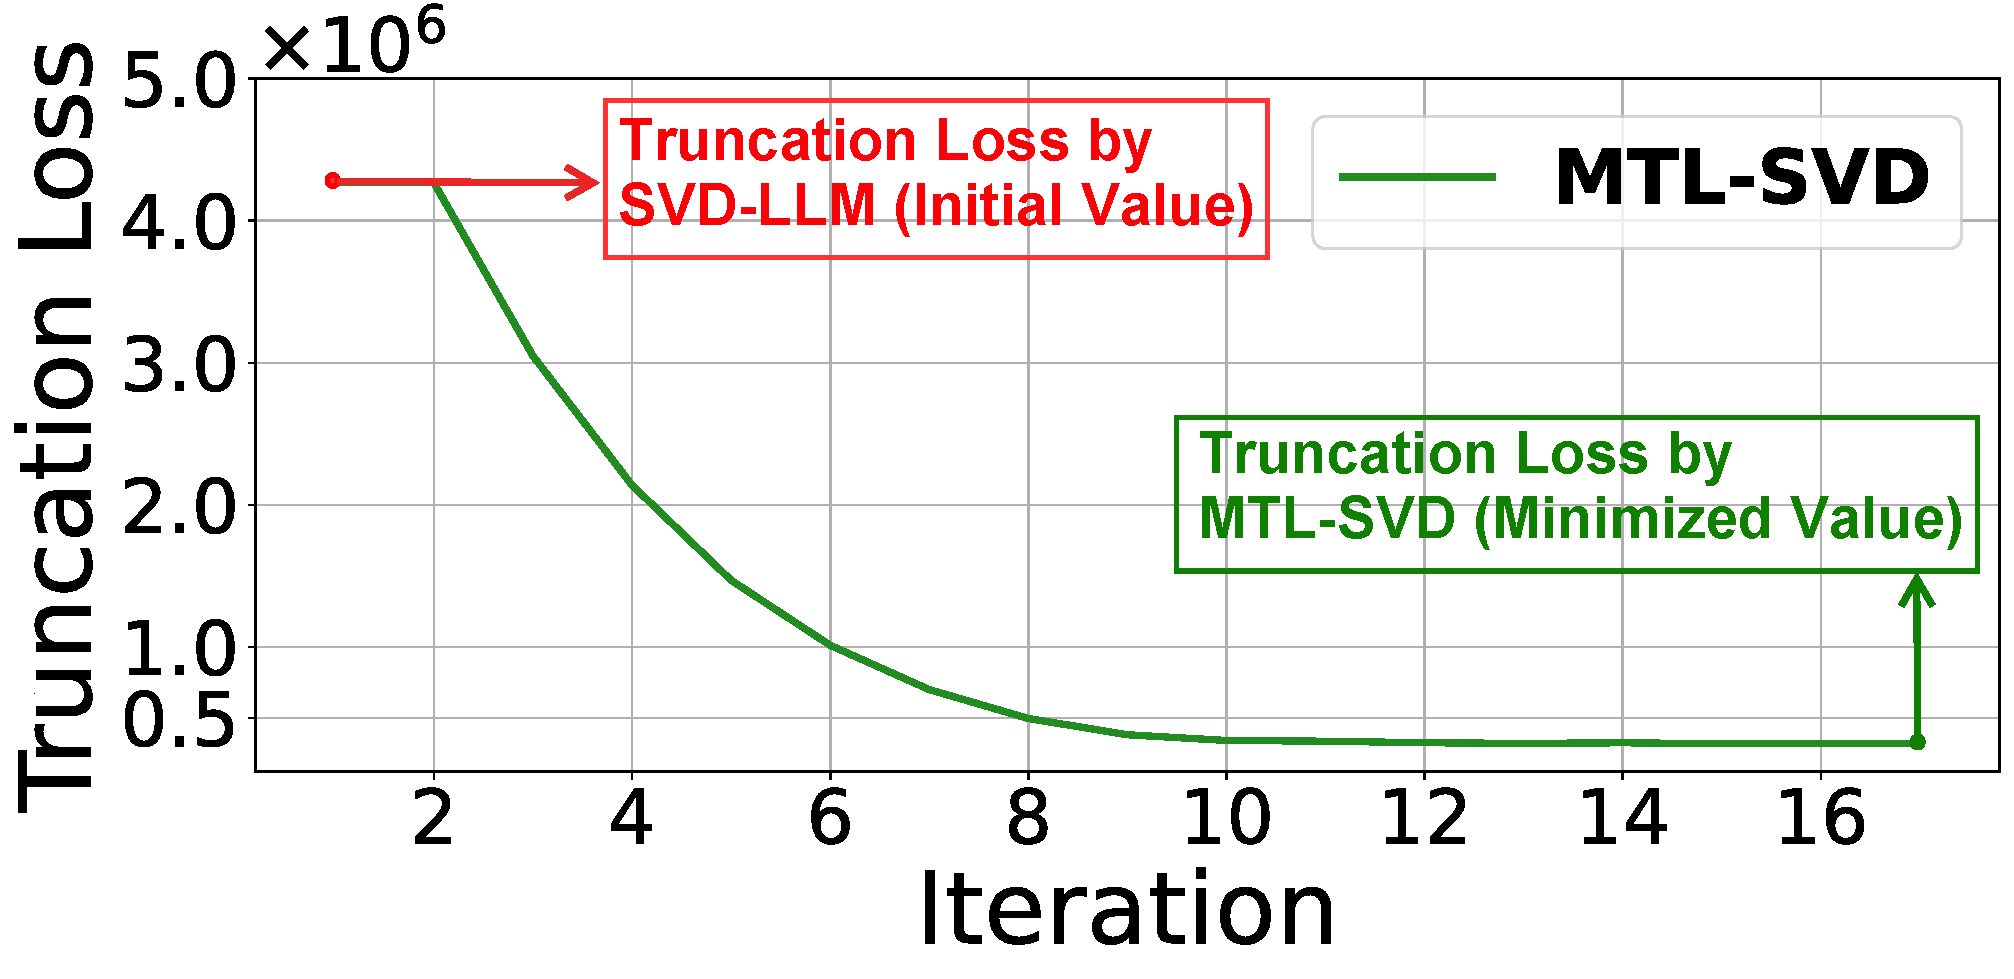
\includegraphics[width=0.45\textwidth]{Figures/Gradient.pdf}
%     \caption{Truncation loss (upper-bound) of the weight matrix in LLaMA-3 8B during the optimization process.}
%     \label{fig:gradient}
%     % % \vspace{-2mm}
% \end{figure}

% To further improve the optimization efficiency, we initialize $M$ to identity matrix, i.e., $M = I$. Therefore, the initial truncation loss is $\sqrt{\sum_{i=1}^r\sigma_i^2}$, which is exactly equal to the truncation loss obtained by SVD-LLM. For a better demonstration, we randomly select one weight matrix in LLaMA-3 8B and plot its upper-bound truncation loss during the optimization process. As shown in~\cref{fig:gradient}, the truncation loss drops significantly via optimization, 
% demonstrating the effectiveness of our proposed loss-minimized weight truncation strategy.


\section{Experiments and Analysis}
\label{sec:experiments}
\accuracyTable
\textbf{Baselines.} 
We compare \sysname against two groups of methods. (1) Three state-of-the-art SVD-based LLM compression methods: FWSVD~\citep{DBLP:conf/iclr/HsuHCLSJ22}, ASVD~\citep{DBLP:journals/corr/abs-2312-05821}, and SVD-LLM~\citep{DBLP:journals/corr/abs-2403-07378} (Section~\ref{subsec:overall_performance}). (2) Other types of LLM compression methods. These include three state-of-the-art pruning-based LLM compression methods: LLM-Pruner~\citep{DBLP:conf/nips/MaFW23}, SliceGPT~\citep{DBLP:conf/iclr/AshkboosCNHH24}, and BlockPruner~\citep{DBLP:journals/corr/abs-2406-10594}, and two state-of-the-art quantization-based LLM compression methods: PB-LLM~\citep{DBLP:conf/iclr/YuanSD24}, and BiLLM~\citep{DBLP:conf/icml/HuangLQLZ0M024} (Section~\ref{subsection:Comparison_with_other_compression_methods}).

\vspace{1mm}
\noindent\textbf{Models and Datasets.} To demonstrate the generability of our method, we evaluate the performance of \sysname on five models at various scales (LLaMA-7B, 13B, 30B, LLaMA3-8B~\citep{DBLP:journals/corr/abs-2307-09288}, OPT-6.7B~\citep{DBLP:journals/corr/abs-2205-01068}) and ten datasets including two language modeling datasets (WikiText-2~\citep{DBLP:conf/iclr/MerityX0S17} and C4~\citep{DBLP:journals/jmlr/RaffelSRLNMZLL20}), six classification datasets (OpenbookQA~\citep{DBLP:conf/emnlp/MihaylovCKS18}, WinoGrande~\citep{DBLP:conf/aaai/SakaguchiBBC20}, HellaSwag~\citep{DBLP:conf/acl/ZellersHBFC19}, Arc\_e~\citep{DBLP:journals/corr/abs-1803-05457}, PIQA~\citep{DBLP:conf/aaai/BiskZLGC20}, MathQA~\citep{DBLP:conf/naacl/AminiGLKCH19}),  and two generation datasets (TruthfulQA~\citep{DBLP:conf/acl/LinHE22} and GSM8K~\citep{DBLP:journals/corr/abs-2110-14168})  with the LM-Evaluation-Harness framework~\citep{eval-harness}.

\vspace{1mm}
\noindent\textbf{Implementation Details.} 
We randomly select $256$ WikiText-2 samples as the calibration data. To mitigate the error raised by the Choleksy decomposition in SVD-LLM due to positive definite, we followed the implementation of SVD-LLM~\citep{DBLP:journals/corr/abs-2403-07378} to add the small noise into the decomposed matrices. The compression ration in our experiments refers to the parameter reduction of LLM achieved through compression. All of the experiments are conducted on A100 GPUs.

\subsection{Performance Comparison}
\label{subsec:overall_performance}
%To examine the generability of \sysname, 
We first compare \sysname against state-of-the-art SVD-based LLM compression methods from four aspects: (1) performance on different LLMs, (2) performance on LLMs with larger scales, (3) performance under different compression ratios, and (4) compression speed.

\vspace{1mm}
\noindent\textbf{Performance on Different LLMs.} 
We compare the performance between \sysname and the baselines on three different LLMs, including LLaMA-7B, OPT-6.7B, and LLaMA-3 8B  under 20\% compression ratio on ten datasets. As shown in~\cref{tab:dataset_acc},  \sysname consistently achieves better and more stable performance than all the SVD-based LLM compression baselines across all three LLMs and all ten datasets. 
%
In particular, \sysname achieves up tp 42\% perplexity reduction and 9\% accuracy
improvement with better generation ability compared to prior state-of-the-art method SVD-LLM on LLaMA-3 8B.

\vspace{1mm}
\noindent\textbf{Performance on LLMs with Larger Scales.} 
We compare the performance between \sysname and the baselines on LLaMA-13B and LLaMA-30B under 20\% compression ratio on WikiText-2 and six classification datasets. As shown in~\cref{tab:large_llm_acc}, \sysname consistently outperforms all the baselines on both 13B and 30B model sizes. 


\largellmaccuracyTable

\vspace{1mm}
\noindent\textbf{Performance under Different Compression Ratios.}
We compare the performance between \sysname and the baselines on LLaMA-7B under compression ratio ranging from 20\% to 80\% on WikiText-2 and six classification datasets. As shown in~\cref{fig:ratio}, \sysname consistently outperforms all baselines, and the performance gain compared to the best-performing baseline increases as the compression ratio increases. 

\vspace{1mm}
\noindent\textbf{Compression Speed.}
Besides measuring the performance of the compressed LLMs, we also evaluate the compression speed. Specifically, we measure the A100 GPU hours used by \sysname and the baseline methods for compressing LLaMA-7B under 20\% compression ratio. 
%
Our results show that FWSVD takes about 6 GPU hours, ASVD takes about 5.5 GPU hours, SVD-LLM takes about 15 minutes, and \sysname takes about 18 minutes to finish the compression. 
%
FWSVD requires gradient calculation, thus consumes a significant amount of time for compression. 
%
For the other methods, the main reason for such a variation is their respective techniques for allocating compression ratios among weight matrices. SVD-LLM assigns the same compression ratio to all weight matrices, enabling the fastest operation but sacrificing accuracy. ASVD, however, determines the compression ratio by regularly evaluating the end-to-end perplexity, which slows down its compression process. In contrast, \sysname allocates the compression ratio directly from its truncation loss, making it significantly faster than ASVD.


\begin{figure}[t]
    \begin{subfigure}{0.48\textwidth}
            \centering
            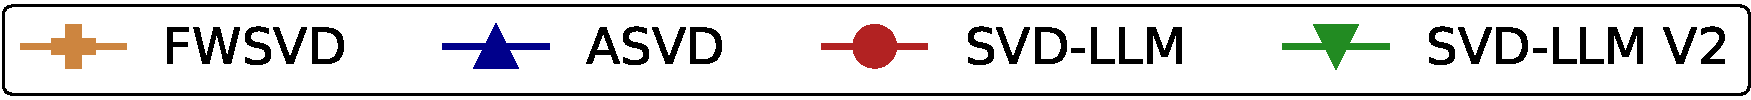
\includegraphics[width=\linewidth]{Figures/ratio_legend.pdf}
            % \vspace{1mm}
        \end{subfigure}
        \\
         \begin{subfigure}{0.235\textwidth}
            \centering
            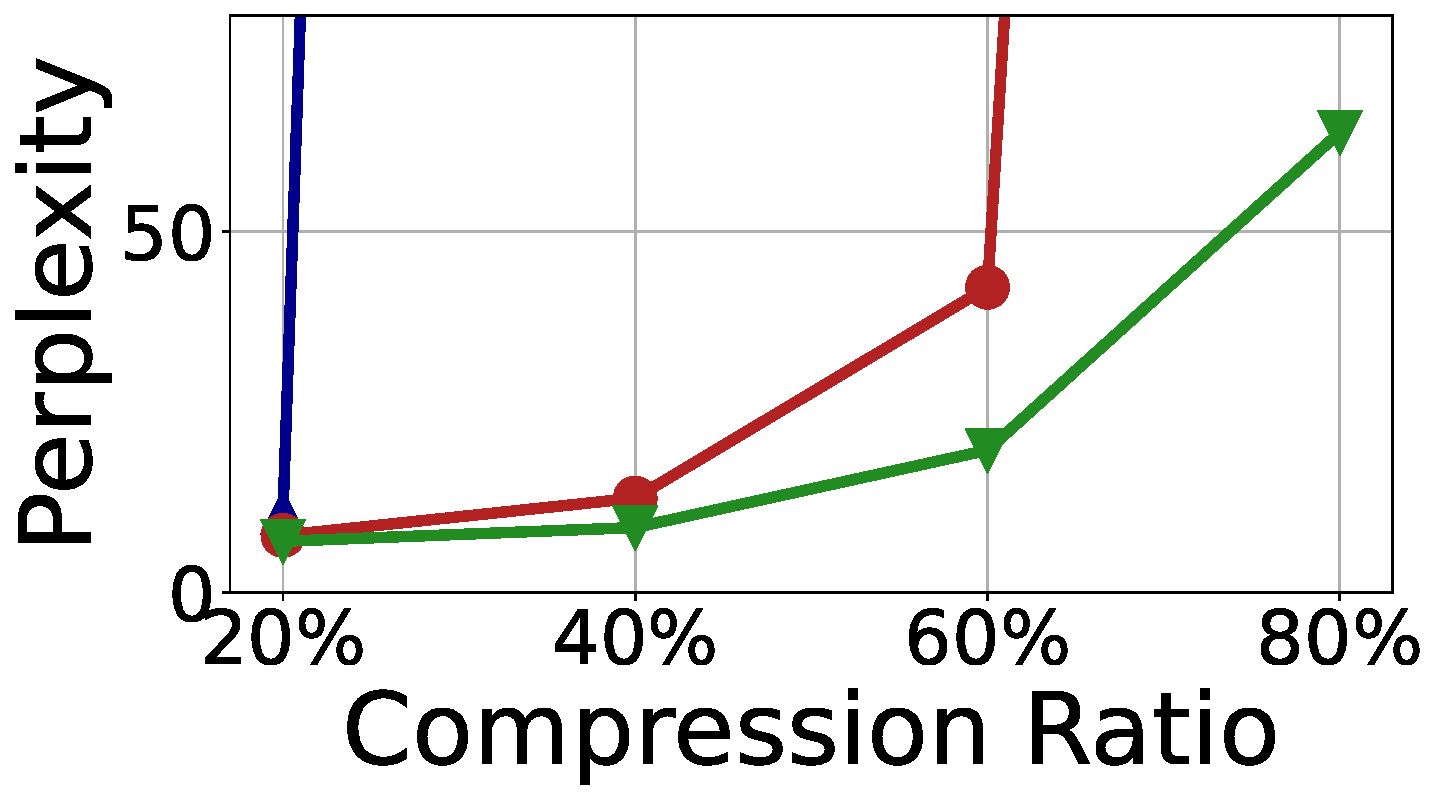
\includegraphics[width=\linewidth]{Figures/ppl_ratio.pdf}  % 插入图像
            \caption{Perplexity}
            \label{fig:ppl_ratio}
        \end{subfigure}
        \begin{subfigure}{0.235\textwidth}
            \centering
            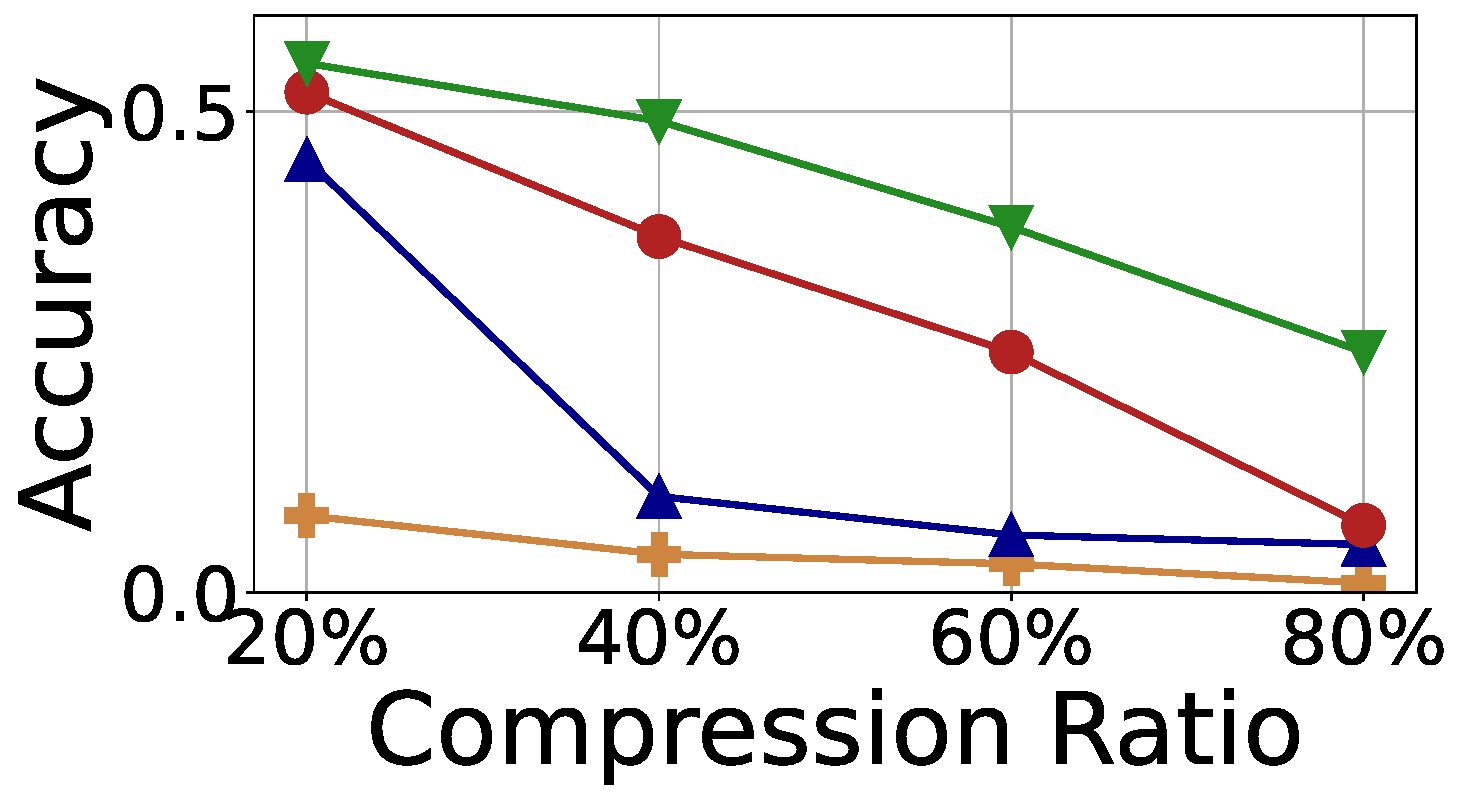
\includegraphics[width=\linewidth]{Figures/acc_ratio.pdf}  % 插入图像
            \caption{Average Accuracy}
            \label{fig:acc_ratio}
        \end{subfigure}
\caption{Perplexity on WikiText-2 and average accuracy on six classification datasets of LLaMA-7B compressed by \sysname  and other SVD-based LLM compression baselines under 20\% to 80\% compression ratios. The perplexity values of FWSVD and ASVD are larger than 100, thus are not shown in the figure.}
\vspace{-5mm}
\label{fig:ratio}
\end{figure}

\subsection{Inference Speedup of \sysname }
\label{subsec:inference_speedup}
% \vspace{-2mm}
To evaluate the inference speedup of models compressed by \sysname, we measure the numbers of tokens generated per second from both the original LLaMA-7B and the model compressed by \sysname under different compression ratios on a single NVIDIA A100 GPU. 
%
For a fair comparison, we fix the batch size to 4, the prefill length to 1024,  and the decoding length to 256. As shown in~\cref{fig:speedup}, \sysname consistently achieves faster token generation speeds across all the compression ratios. 
%
More importantly, the speedup becomes more significant as the compression ratio increases, resulting in a speedup of 1.29x under 20\% compression ratio, 1.63x under 40\% compression ratio, 2.08x under 60\% compression ratio, and 2.71x under 80\% compression ratio. 

% \vspace{-2mm}
\begin{figure}[t]
    \centering
    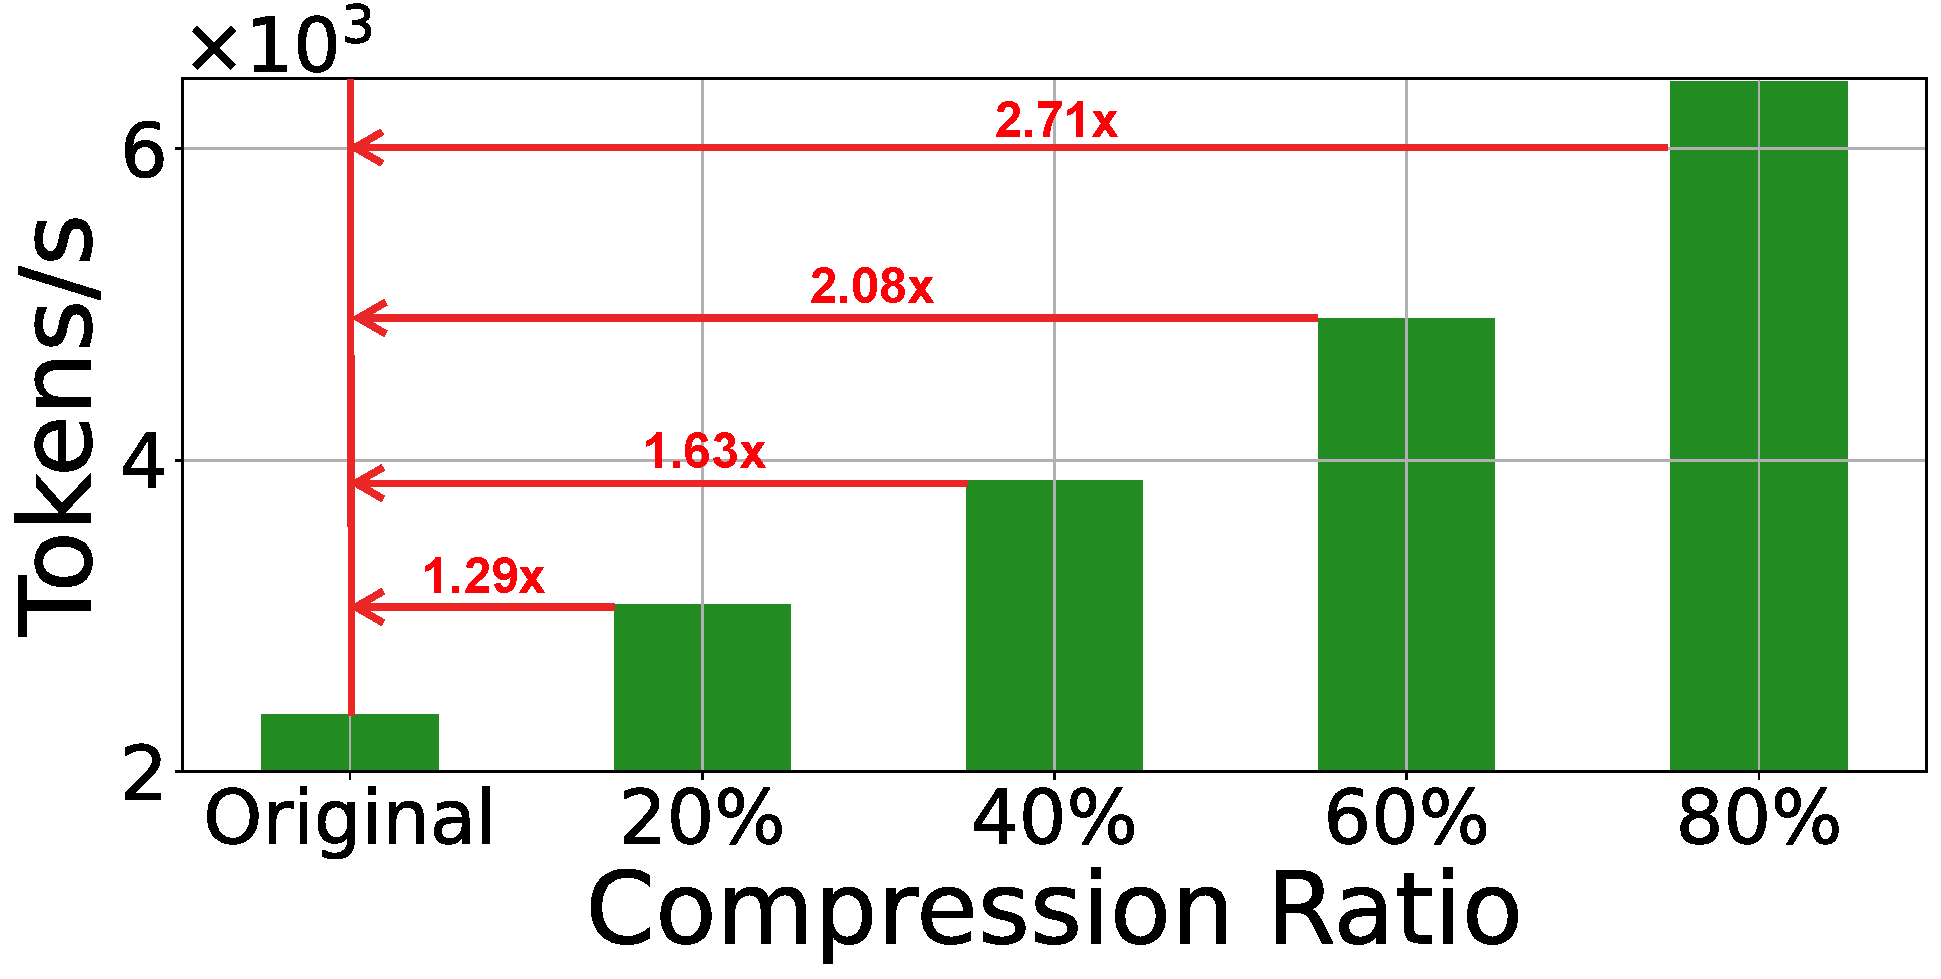
\includegraphics[width=0.4\textwidth]{Figures/Speedup.pdf}
    \caption{Throughput (Tokens/s) achieved by original LLaMA-7B and its compressed version by \sysname under different compression ratios on a single NVIDIA A100 GPU. We fix the batch size to 4, prefill length to 1024,  and decoding length to 256.  The speedup over the original LLM is marked in red.}
    \label{fig:speedup}
    % \vspace{-10mm}
\end{figure}

\vspace{2mm}
\sensitivityTable

\subsection{Ablation Study}
\label{subsec:ablation_study}
\sysname has two key components, both of which optimize the truncation loss. 
%
In our ablation study, we first evaluate the individual contribution of each of the two components to the compression performance. 
%
Next, since both components fully utilize the whitening matrix $S$, which is calculated with a randomly selected calibration set, we evaluate the impacts of different calibration data on the performance of \sysname.

\vspace{1mm}
\noindent\textbf{Component Sensitivity Study.} We first evaluate the individual contribution of the two components (i.e., heterogeneous compression ratio allocation and loss-optimized weight truncation) of \sysname. 
%
Let \sysname (A) denote the version of \sysname with heterogeneous compression ratio allocation only; and \sysname (T) denote the version of \sysname with loss-optimized weight truncation only.
%; and \sysname (A+T) denote the version of \sysname with both heterogeneous compression ratio allocation and loss-optimized weight truncation.
%
The results are shown in~\cref{tab:sensitivity}. We have two observations. 
%
(1) Both \sysname (A) and \sysname (T) outperform SVD-LLM, demonstrating the effectiveness of each of these two components alone in achieving superior compression performance.
%
(2) \sysname outperforms \sysname (A) and \sysname (T), demonstrating the necessity of having both components.

\vspace{1mm}
\noindent\textbf{Impact of Calibration Set.} Next, we examine the impact of the calibration set on the compression performance of \sysname. Specifically, we measure the changes in perplexity of LLaMA-7B compressed by \sysname under 20\% compression ratio on WikiText-2 when using the default calibration set but with various numbers of data and sampling seeds.
%
As shown in~\cref{fig:calibration}, the changes in both data number and sampling seed in the calibration set incur no more than 1\% fluctuation in the final performance, demonstrating that \sysname is not sensitive to the calibration set.

\begin{figure}[t]
         \begin{subfigure}{0.235\textwidth}
            \centering
            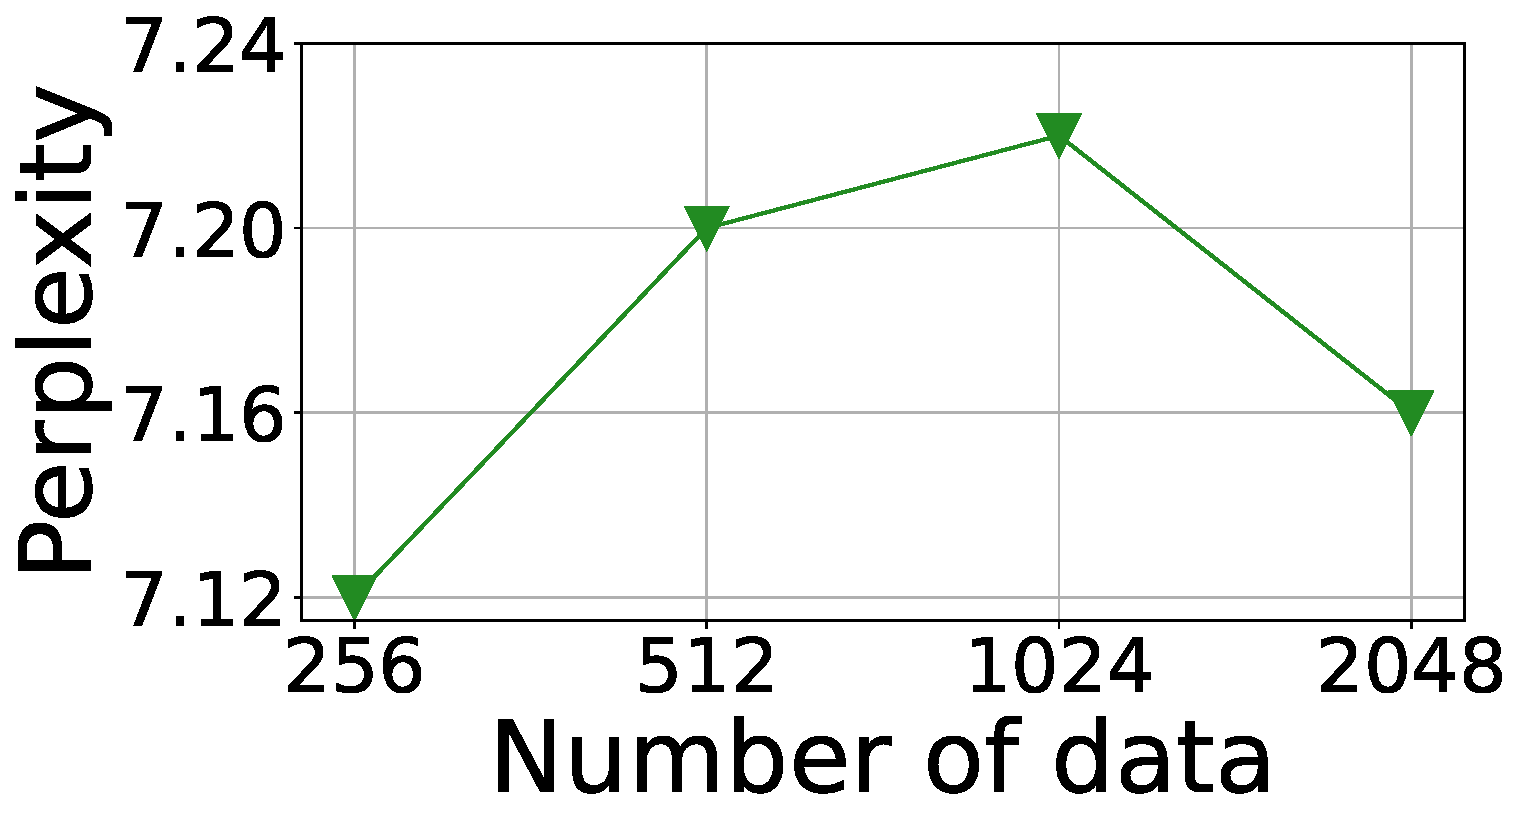
\includegraphics[width=\linewidth]{Figures/cali_size.pdf}  % 插入图像
            \caption{Various Data Number}
            \label{fig:cali_number}
        \end{subfigure}
        \begin{subfigure}{0.24\textwidth}
            \centering
            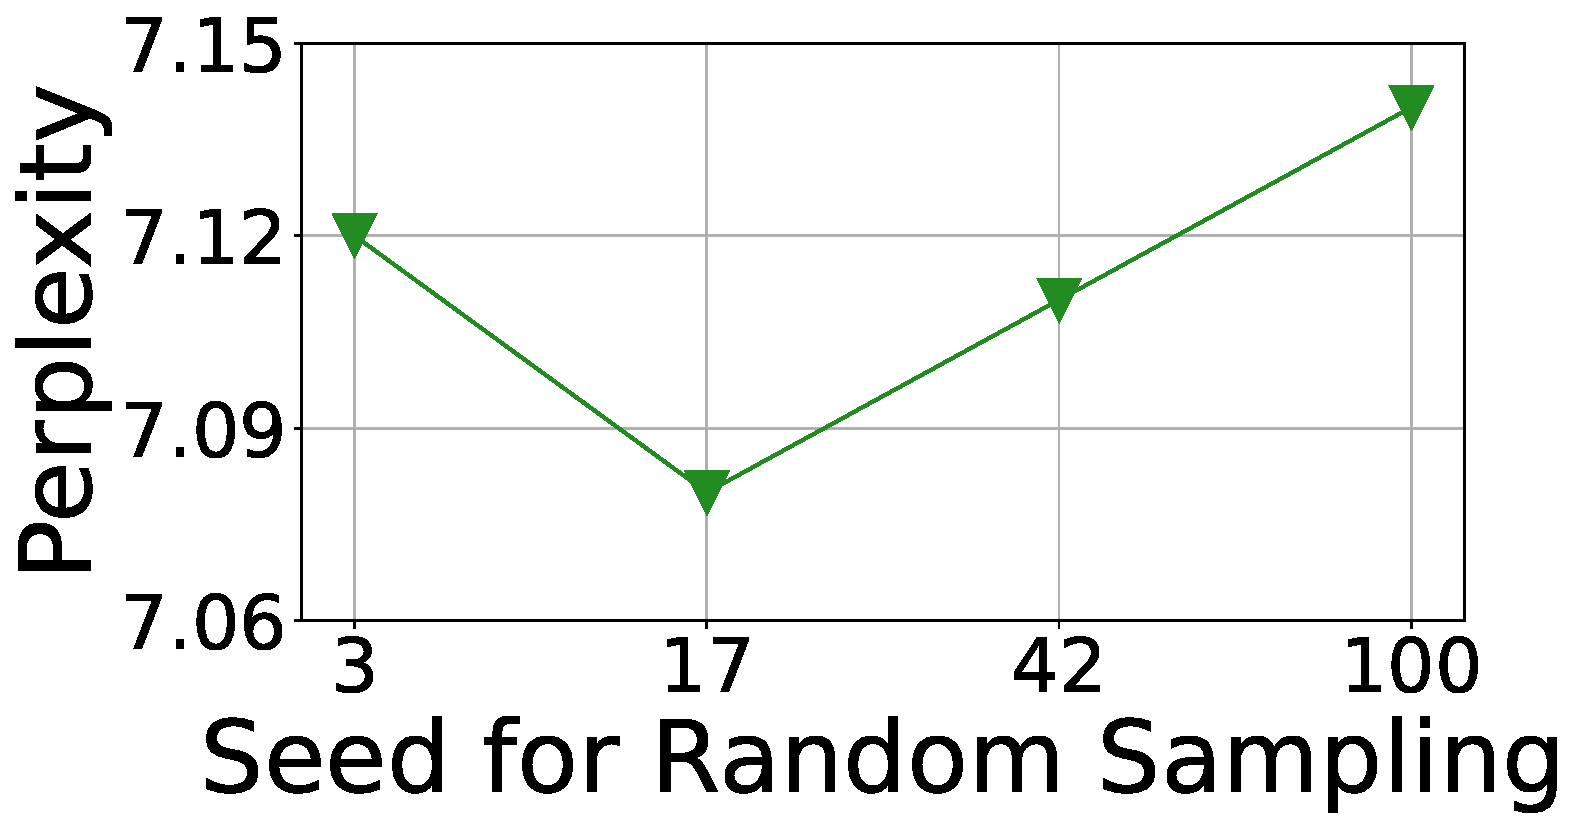
\includegraphics[width=\linewidth]{Figures/seed.pdf}  % 插入图像
            \caption{Various Samping Seed}
            \label{fig:cali_seed}
        \end{subfigure}
\caption{Perplexity of LLaMA-7B under 20\% compression ratio using calibration data sampled with different numbers or seeds from WikiText-2.}
\label{fig:calibration}
\end{figure}

\subsection{Comparison with Other Types of Post-training LLM Compression Methods} 
\sysname is orthogonal to other post-training LLM compression methods, including quantization and pruning. In this experiment, we compare the performance of \sysname with state-of-the-art structured pruning-based and quantization-based LLM compression methods. 

\svdprunepplTable

% \vspace{-8mm}
\svdpruneaccTable

\noindent\textbf{Comparison with Structured Pruning.}
First, we compare \sysname with three state-of-the-art post-training structured pruning-based LLM compression methods: LLM-Pruner~\citep{DBLP:conf/nips/MaFW23}, SliceGPT~\citep{DBLP:conf/iclr/AshkboosCNHH24}, and BlockPruner~\citep{DBLP:journals/corr/abs-2406-10594} under various weight memory budgets, ranging from 10 GB to 7 GB. 
%
The perplexity results are shown in~\cref{tab:svd_prune_ppl} and the average accuracy results are shown in~\cref{tab:svd_prune_acc}. 
%
As shown, \sysname outperforms all three state-of-the-art structured pruning-based LLM compression methods. In particular, under 7 GB memory budget, \sysname achieves 28\% reduction in perplexity and 13\% higher average accuracy.


\vspace{1mm}
\noindent\textbf{Comparison with Quantization.} 
%
Next, we compare \sysname with post-training quantization-based LLM compression methods. 
%
We first compare \sysname with GPTQ~\citep{DBLP:journals/corr/abs-2210-17323} under 3-bit quantization. As shown in~\cref{tab:svd_quant_4bit}, while \sysname achieves worse perplexity compared to GPTQ under 3-bit memory budget, 
%it still remains highly useful for moderate compression ratios. 
%This is because 
combining \sysname (30\% compression ratio) with GPTQ-4-bit achieves superior perplexity compared to GPTQ-3-bit under the same memory budget. 
%Specifically, because SVD-based compression is orthogonal to and can be seamlessly combined with quantization-based methods, 
In other words, we find that under the same memory budget, by first compressing the original 16-bit LLM with \sysname at 30\% compression ratio, then quantizing the compressed LLM to 4-bit using GPTQ, we are able to achieve better perplexity compared to directly quantizing the original LLM to 3-bit.  
%
Finally, we compare \sysname with  two state-of-the-art post-training quantization-based LLM compression methods: BiLLM~\citep{DBLP:conf/icml/HuangLQLZ0M024} and PB-LLM~\citep{DBLP:conf/iclr/YuanSD24}, which push the frontier to 1-bit quantization.
%under 1-bit quantization. 
%
The results are shown in Table~\ref{tab:svd_quant}. 
%
We have two observations: (1) Without combining with quantization techniques, \sysname (16-bit) outperforms PB-LLM with 5\% lower perplexity.
%
%achieves a performance comparable to several 1-bit post-training quantization methods. In particular, it achieves 5\% lower perplexity than PB-LLM~\citep{DBLP:conf/iclr/YuanSD24}, highlighting the effectiveness of \sysname in compressing LLM to the extremely low memory budge similar to 1-bit quantization. 
%
(2) By combining with quantization techniques, \sysname (2-bit) outperforms state-of-the-art 1-bit post-training quantization method BiLLM. In particular, \sysname (2-bit) achieves 69\% lower perplexity than BiLLM, showing the promise of combining SVD-based and quantization-based compression methods for pushing the frontier of post-training LLM compression forward.
%a new research avenue that combines \sysname with recent quantization methods to further enhance compression performance.


\vspace{0mm}
\svdquanthighTable

\vspace{0mm}
\svdquantTable

\label{subsection:Comparison_with_other_compression_methods}
\vspace{-1mm}
\section{Conclusion}
\label{sec:conclusion}

\vspace{-2mm}
In this paper, we present \sysname, a SVD-based post-training LLM compression method. \sysname addresses the limitation of existing methods about high truncation loss during compression. Specifically, \sysname first employs a heterogeneous compression ratio allocation strategy to effectively balance truncation loss across different weight matrices of the LLM. It further introduces a loss-optimized weight truncation to ensure a lower and more stable truncation loss. 
% We evaluated \sysname on 10 datasets and five models at three scales. Our results demonstrate the superiority of \sysname over state-of-the-arts.
Our evaluation results demonstrate the superiority of \sysname over state-of-the-art SVD-based post-training LLM compression methods.

% Bibliography entries for the entire Anthology, followed by custom entries
%\bibliography{anthology,custom}
% Custom bibliography entries only
\vspace{-1mm}
\section{Limitations}
\vspace{-1mm}

While \sysname outperforms existing SVD-based LLM compression methods, there is still space for further improvement. For example, under 90\% compression ratio, there is a small performance gap compared with state-of-the-art quantization methods.
%
We aim to fill this gap in future.

\vspace{-1mm}
\section{Acknowledgement}
\vspace{-1mm}

This study is supported in part by NSF Award NeTS-2312675.

\newpage
\bibliography{Reference}
% \newpage
% \appendix
% \section{Appendix}
\label{sec:appendix}
\subsection{Compression Speed Analysis}
\label{appendix:compression_speed_analysis}
Apart from measuring the compressed LLMs' performance, we also evaluate the compression speed of \sysname and the baselines, including ASVD and SVD-LLM. Specifically, we measured the A100 GPU hours used for \sysname and the baseline methods when compressing LLaMA-7B under 20\% compression ratio. The results show that ASVD takes about 5.5 GPU hours, SVD-LLM takes about 15 minutes, while \sysname takes about 1.5 GPU hours to run the compression. Since \sysname not only requires computing the whitening matrices, which consumes the majority of time in SVD-LLM, but also needs to run its own key modules during compression, it is expected to consume longer time than SVD-LLM. However, it is still faster than ASVD, indicating that its compression time is still acceptable for post-training LLM compression. Moreover, our time breakdown analysis shows that the heterogeneous compression ratio allocation only requires 2 minutes, while the loss-minimized weight truncation takes up almost all 1.5 hours. Although this module is time-consuming, it deserves the time cost, as it helps \sysname significantly reduce its truncation loss during the SVD compression.

\subsection{Optimization Details}
\label{appendix:optimization_details}
In our experiments, we use the L-BFGS~\citep{Nash1991ANS} algorithm to perform optimization in loss-minimized weight truncation due to its benefits for fast convergence, especially when dealing with large-scale problems. We set the learning rate to 0.01 and the maximum iteration to 40. Our empirical results show that the loss drops rapidly and often converges in 20 iterations. Therefore, the time consumed to perform this optimization is still acceptable. As mentioned in~\cref{appendix:compression_speed_analysis}, it only takes about 1.5 hours to optimize all weight matrices in LLaMA-7B, which also meets our initial goal of designing an efficient and practical way to minimize truncation loss.


\end{document}
